\documentclass[a4paper,10pt]{article}
\usepackage[utf8]{inputenc}
\usepackage{graphicx}
\usepackage[margin=1.5in]{geometry}
\usepackage{lipsum}
\usepackage{amsmath}
\usepackage{caption}
\usepackage{subcaption}
\usepackage[]{algorithmic}
\usepackage{courier}
\usepackage{float}



%opening
\title{Assignment 4: Markov Decision Processes and Reinforcement Learning}
\author{Brent Mitton}

\begin{document}

\maketitle

\section{Abstract}
This paper is a brief look at some simple reinforcement learning techniques as applied to Markov decision processes (MDPs). There will be a focus on three different methods of reinforcement learning and a comparison of how these methods perform on two toy problems.

\section{Introduction}
\subsection{Techniques}
This paper will look at three different algorithms for reinforcement learning on Markov decision processes. The first two of these models are policy iteration and value iteration. These two techniques aim to find the optimal policy, $\pi^*$, of an MDP given that they are provided a  model of the MDP. For the purposes of this paper a \textit{model} means a transition matrix, $T(s, a, s')$, and a reward matrix $R(s, a)$. The transition matrix gives the probability of ending up in state $s'$, give that the agent was in state $s$ and took action $a$. The reward matrix returns the reward achieved from being in state $s$ and taking action $a$. 

The third technique that will be looked at is called Q-learning. This is one technique that aims to learn the optimal policy of the MDP without being given a model. This sort of method is often more suitable to real-world problems where we don't have prior knowledge of the transition and reward functions, but instead want the agent to learn and react to environmental stimulus.

\subsubsection{Value and Policy Iteration}
The aim of value iteration is to find the optimal value function, $V^*(s)$, of the MDP. Then, by using the discovered optimal value function the optimal policy can be inferred. The optimal value function of an MDP is defined as:

\begin{equation}
V^*(s) = \underset{a}{max} (R(s,a) + \gamma \sum\limits_{s' \in S} T(s, a, s') V^*(s')), \forall s\in S
\end{equation}

The value of a state is the immediate reward of being in the state plus the expected discounted reward of following the optimal path (path of highest reward) from that point on. The optimum policy, $\pi^*$, of an MDP can be inferred given $V^*(s)$:


\begin{equation}
\pi^*(s) = \underset{a}{argmax}(R(s,a) + \gamma \sum\limits_{s' \in S} T(s,a,s') V^*(s'))
\end{equation}

Using a simple iterative process, we can find the correct $V^*(s)$ of an MDP, and thus are able to find the optimal policy. [1]\\

\begin{algorithmic}[H]
\scriptsize
\ttfamily
  \STATE intialize all V(s) arbitrarily
  \REPEAT
  	\FORALL{$s \in S$}
		\FORALL{$a \in A$}
			\STATE $Q(s,a) \leftarrow R(s,a) + \gamma \sum\limits_{s'  \in S} T(s, a, s') V(s')$
		\ENDFOR
		\STATE $V(s) \leftarrow \underset{a}{max}Q(s,a)$
	\ENDFOR
  \UNTIL{policy is satisfactory} 
\end{algorithmic}

Policy iteration works by trying to find the optimal policy directly instead of relying on finding the correct value function and then inferring the correct policy.\\

\begin{algorithmic}[H]
\scriptsize
\ttfamily
\STATE choose arbitrary $\pi^*$
\REPEAT
	\STATE $\pi \leftarrow \pi^* $
	\STATE  // Find the value function for current policy by solving systems of linear equations
	\STATE $V_\pi(S) = R(s, \pi(s)) + \gamma \sum\limits_{s' \in S} T(s, a, s') V_\pi(s'), \forall s \in S$
	\STATE // improve the policy at each state
	\STATE $\pi'(s) \leftarrow \underset{a}{argmax}(R(s,a) + \gamma \sum\limits_{s' \in S} T(s, a, s') V_\pi(s'))$
\UNTIL{$ \pi = \pi'$}

\end{algorithmic}

\subsubsection{Q-Learning}
Q-learning works by learning an action-value function $Q(s,a)$ , which is defined to be the expected discounted reward that would be obtained by starting at state $s$, taking action $a$, then continuing optimally from that point. The slightly modified Q-Learning algorithm used for this paper is detailed below.\\

\begin{algorithmic}[H]
\scriptsize
\ttfamily
\STATE initialize Q(s,a) arbitrarily
\STATE initialize $\alpha, \gamma$
\FORALL{episodes}
	\FORALL{$s \in S$}
	\WHILE{ $s \neq$ goalstate}
		\IF{not possible to move from s}
		\STATE // start new episode
		\STATE break
		\ENDIF
		\STATE $a \leftarrow $ action from state using policy derived from Q ($\epsilon$-greedy)
			\STATE $r \leftarrow $ reward from doing $a$
			\STATE $s' \leftarrow $ state after doing $a$
			\STATE $Q(s,a) \leftarrow Q(s,a) + \alpha(r + \gamma \underset{a'}{max}Q(s',a') - Q(s,a)))$
			\IF{New $Q(s,a)$ not significantly different then prior Q(s,a)}
				\STATE // start new episode
				\STATE break
			\ENDIF
			\STATE decrease $\alpha$
			\STATE $ s \leftarrow s'$
			\ENDWHILE

		\ENDFOR
\ENDFOR
\end{algorithmic}

This algorithm is essentially Watkins' Q-Learning algorithm[2] but with a couple of modifications to better suit the problems. 
\begin{enumerate}
\item Ensure that the algorithm does not spend time trying to find best action sequences from states that have no path to the goal.
\item Break into a new episode in the case that $Q(s,a)$ has not changed significantly. This prevents getting stuck in cycles of states, however this may remove the guarantee of convergence.
\end{enumerate}

\subsection{The Problems}
The problems used in this paper to compare the techniques are two different sizes of maze/gridworld problems. The environment for the problem is an NxN grid where each cell is a state. From each cell the agent can take an action $ a \in A $ = \{Go North, Go East, Go South, Go West\}. There are four different types of states to be considered in the environment: 

\begin{itemize}
\item regular states, can be entered from adjacent states
\item wall states, cannot be entered from other states
\item enalty states, give a large negative reward to the the agent
\item goal states, give a large positive reward to the agent and terminates the problem
\end{itemize}

Generally, there is also a step penalty introduced which will give the agent a negative reward for each step taken.
The optimal policy of one of these problems should be the one that maximizes the reward gained.

Gridworlds are an interesting problem to consider for Markov decision processes not only because they are easy to visualize and understand, but also because it is often possible to generalize more complex problems into variants of gridworlds.

\subsubsection{5x5 World}

\begin{figure}[htb!]
\centering
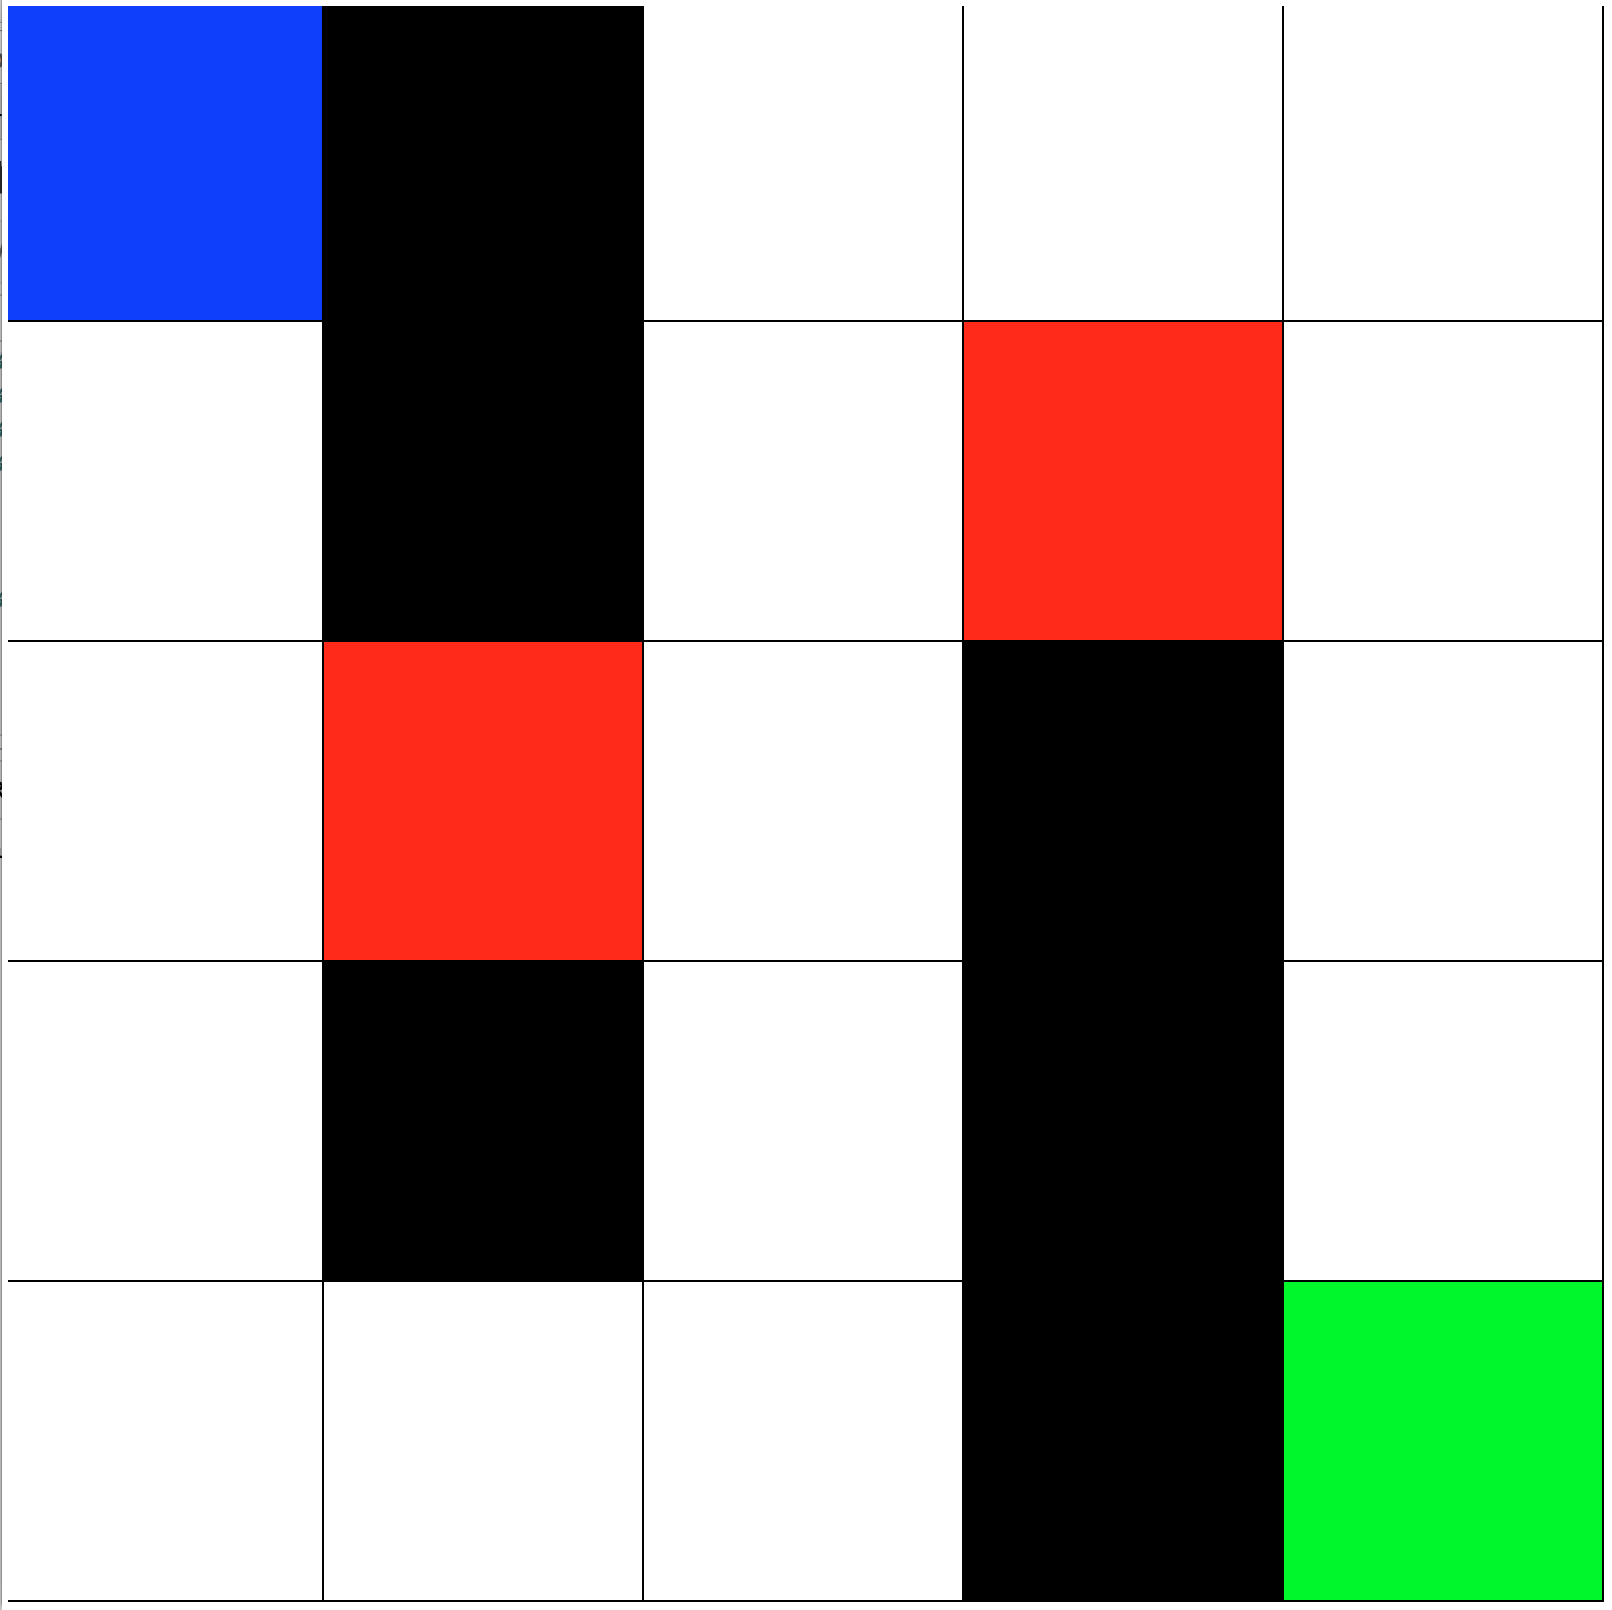
\includegraphics[width=0.5\textwidth]{figures/5by5_nopolicy.png}
\caption{5x5 World}
\end{figure}

The 5x5 gridworld/maze is a small environment used to demonstrate the three techniques. It has a total of 25 possible states that the agent could end up in. Each of the coloured squares in \textit{Figure 1} represents one of the different state types.

\begin{itemize}
\item Blue -- not a state type, indicates the position the agent will start in
\item Black -- a wall state
\item Red -- penalty state
\item Green -- goal state
\end{itemize}

\subsubsection{50x50 World}
\begin{figure}[htb!]
\centering
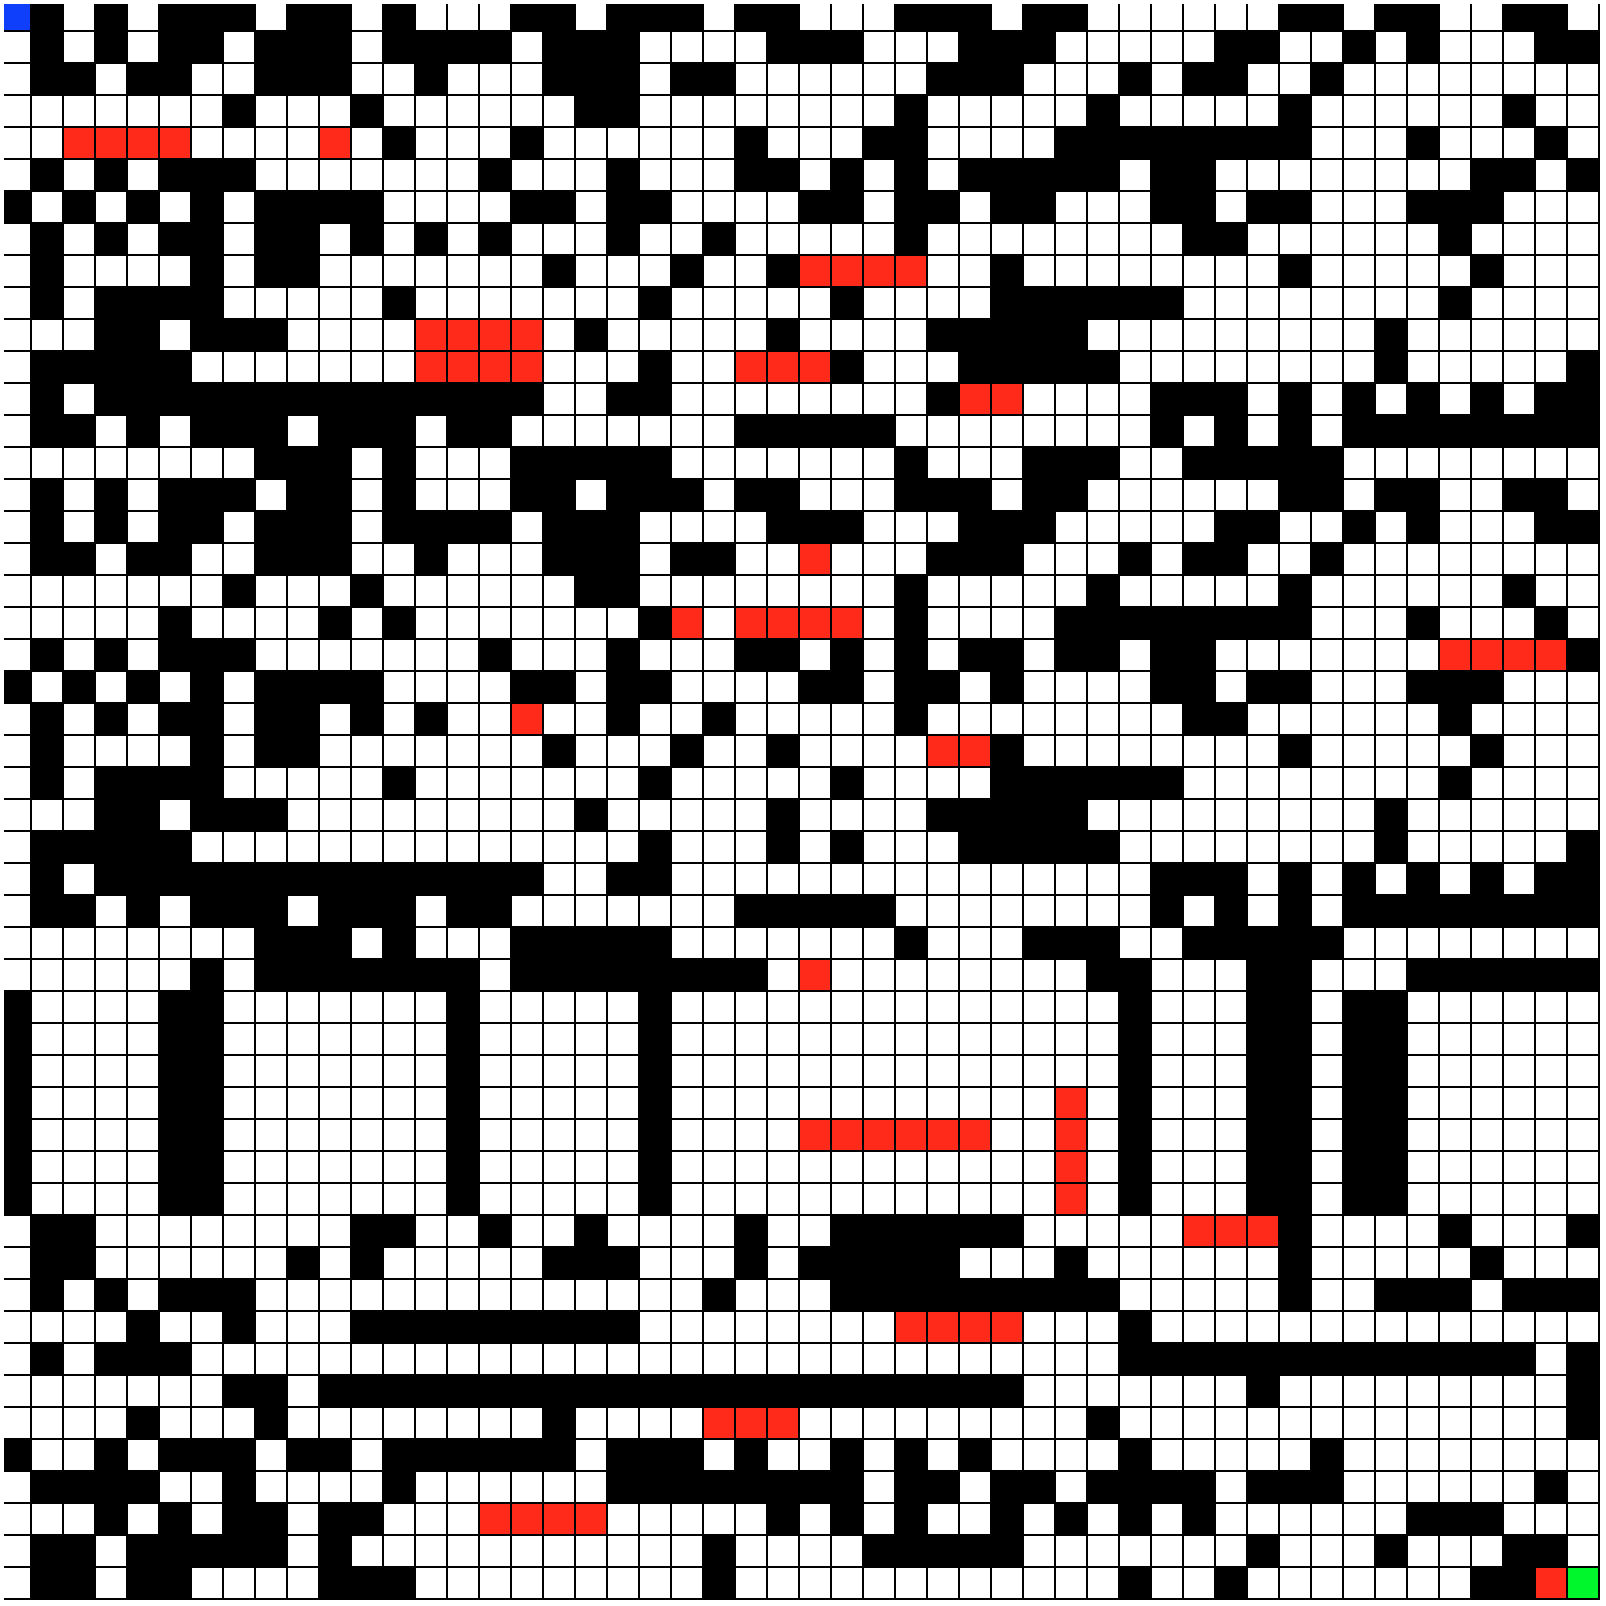
\includegraphics[width=0.5\textwidth]{figures/50by50_nopolicy.png}
\caption{50x50 World}
\end{figure}

The 50x50 gridworld/maze is a larger environment used to demonstrate the three techniques. There are a total of 2500 possible state the agent could end up in. \textit{Figure 2} shows the pseudorandomly generated environment used for experimentation.

\section{Comparisons}
\subsection{5x5 World}
For comparison it is interesting to try each of these methods on different reward schemas. That is, different reward values for: step penalties, entering penalty states, entering the goal states. The reward schema used for applying the three techniques to the 5x5 World will be

\begin{enumerate}
\item Goal State: +10; Step Penalty: -0.05; Penalty State: -1;
\item Goal State: +10; Step Penalty: -1: Penalty State: -5;
\item Goal State: 0; Step Penalty: 1; Penalty State: -2;
\end{enumerate}

\subsubsection{Value Iteration}
\begin{figure}[H]
        \centering
        \begin{subfigure}[b]{0.3\textwidth}
                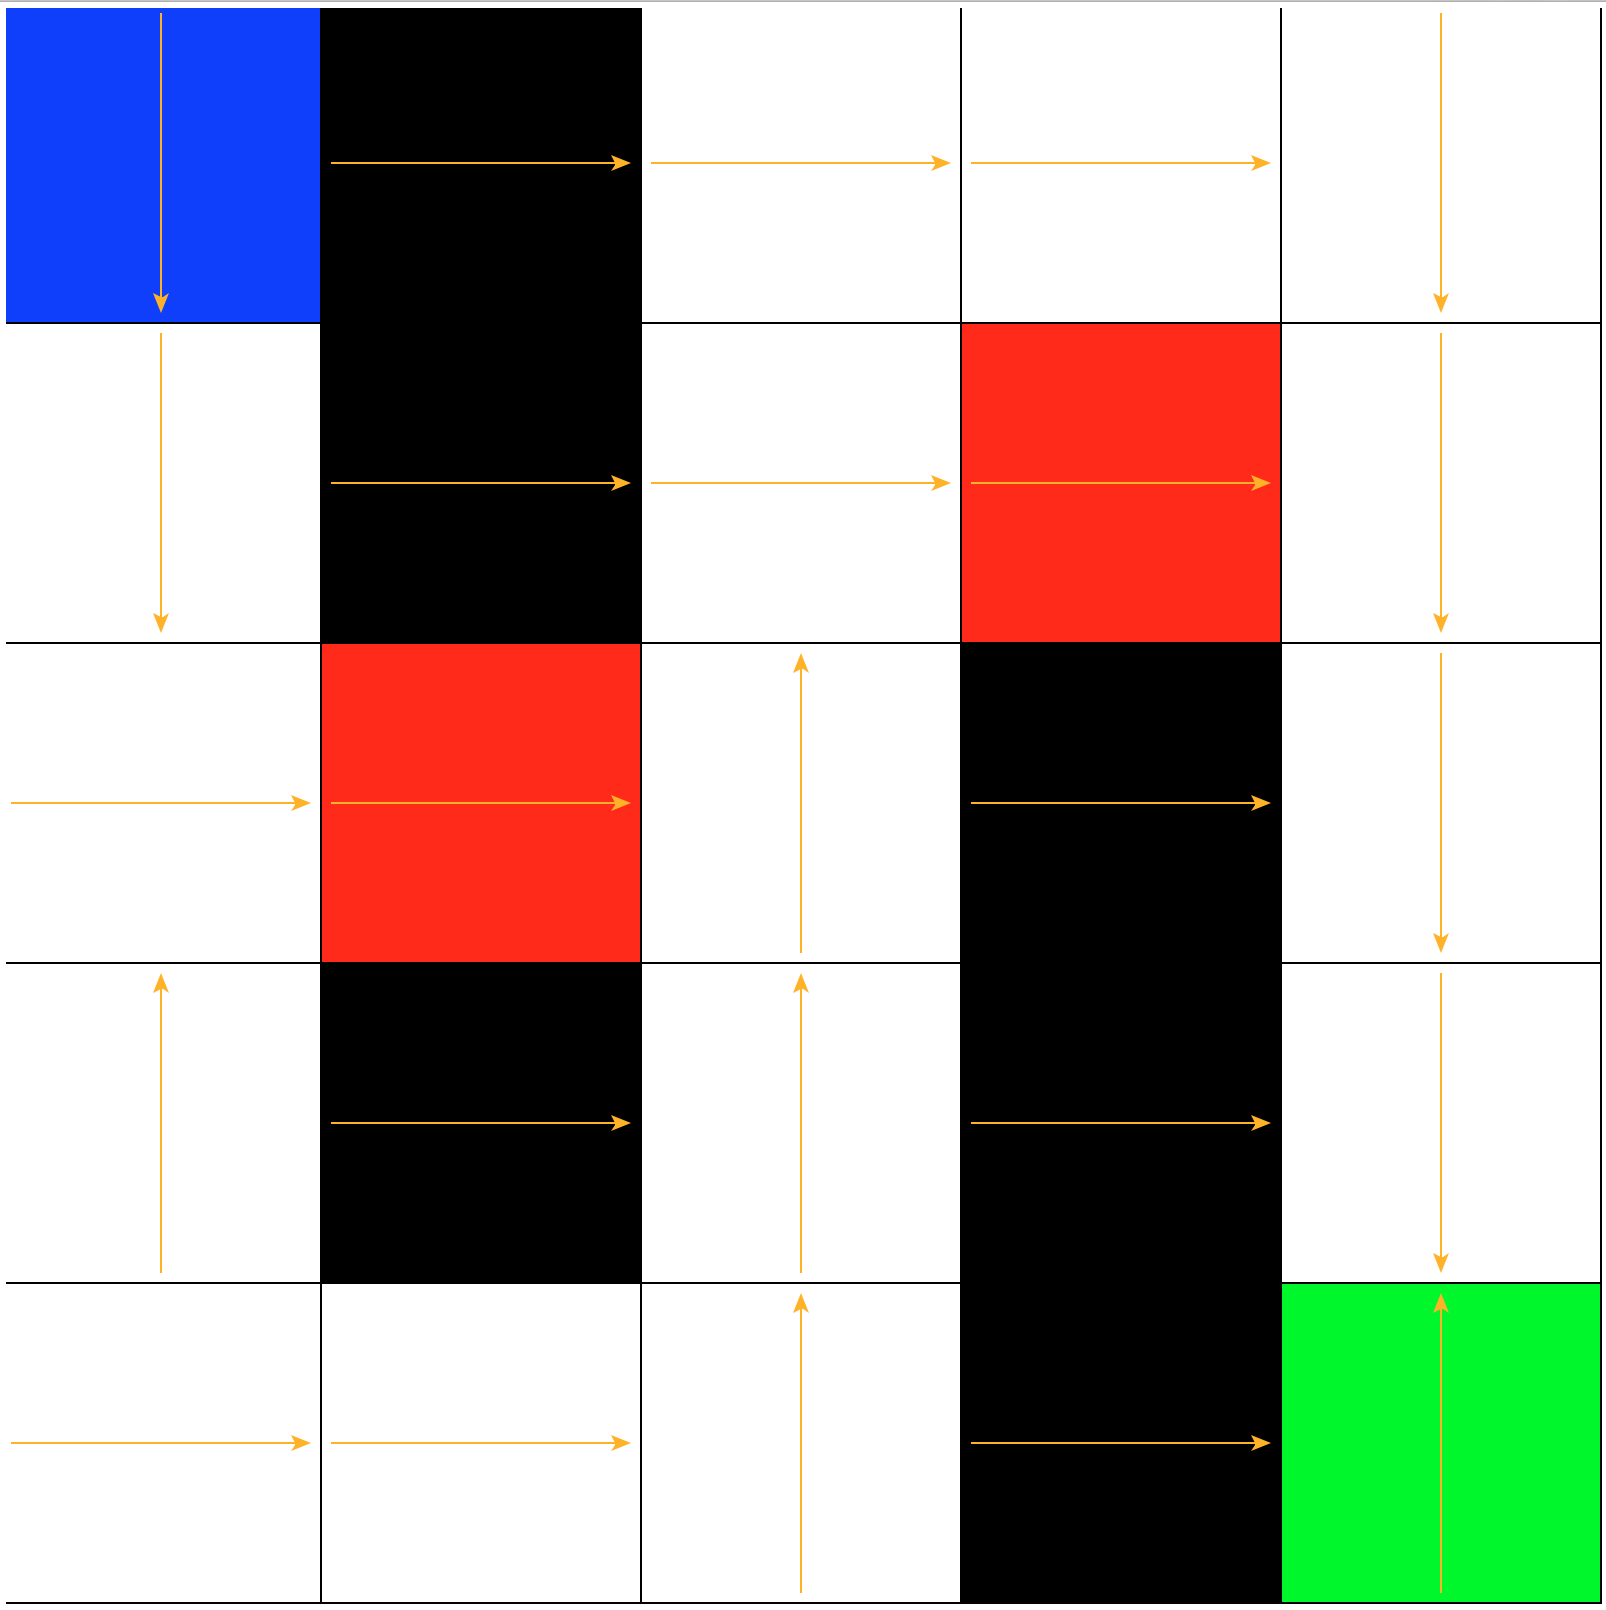
\includegraphics[width=\textwidth]{figures/5x5_viter_r1.png}
                \caption{Reward schema 1\\
                Reward:  7.65\\
                Time:  0.0054\\
                Iterations: 84}
                \label{fig:v1}
        \end{subfigure}%
        ~ %add desired spacing between images, e. g. ~, \quad, \qquad, \hfill etc.
          %(or a blank line to force the subfigure onto a new line)
        \begin{subfigure}[b]{0.3\textwidth}
                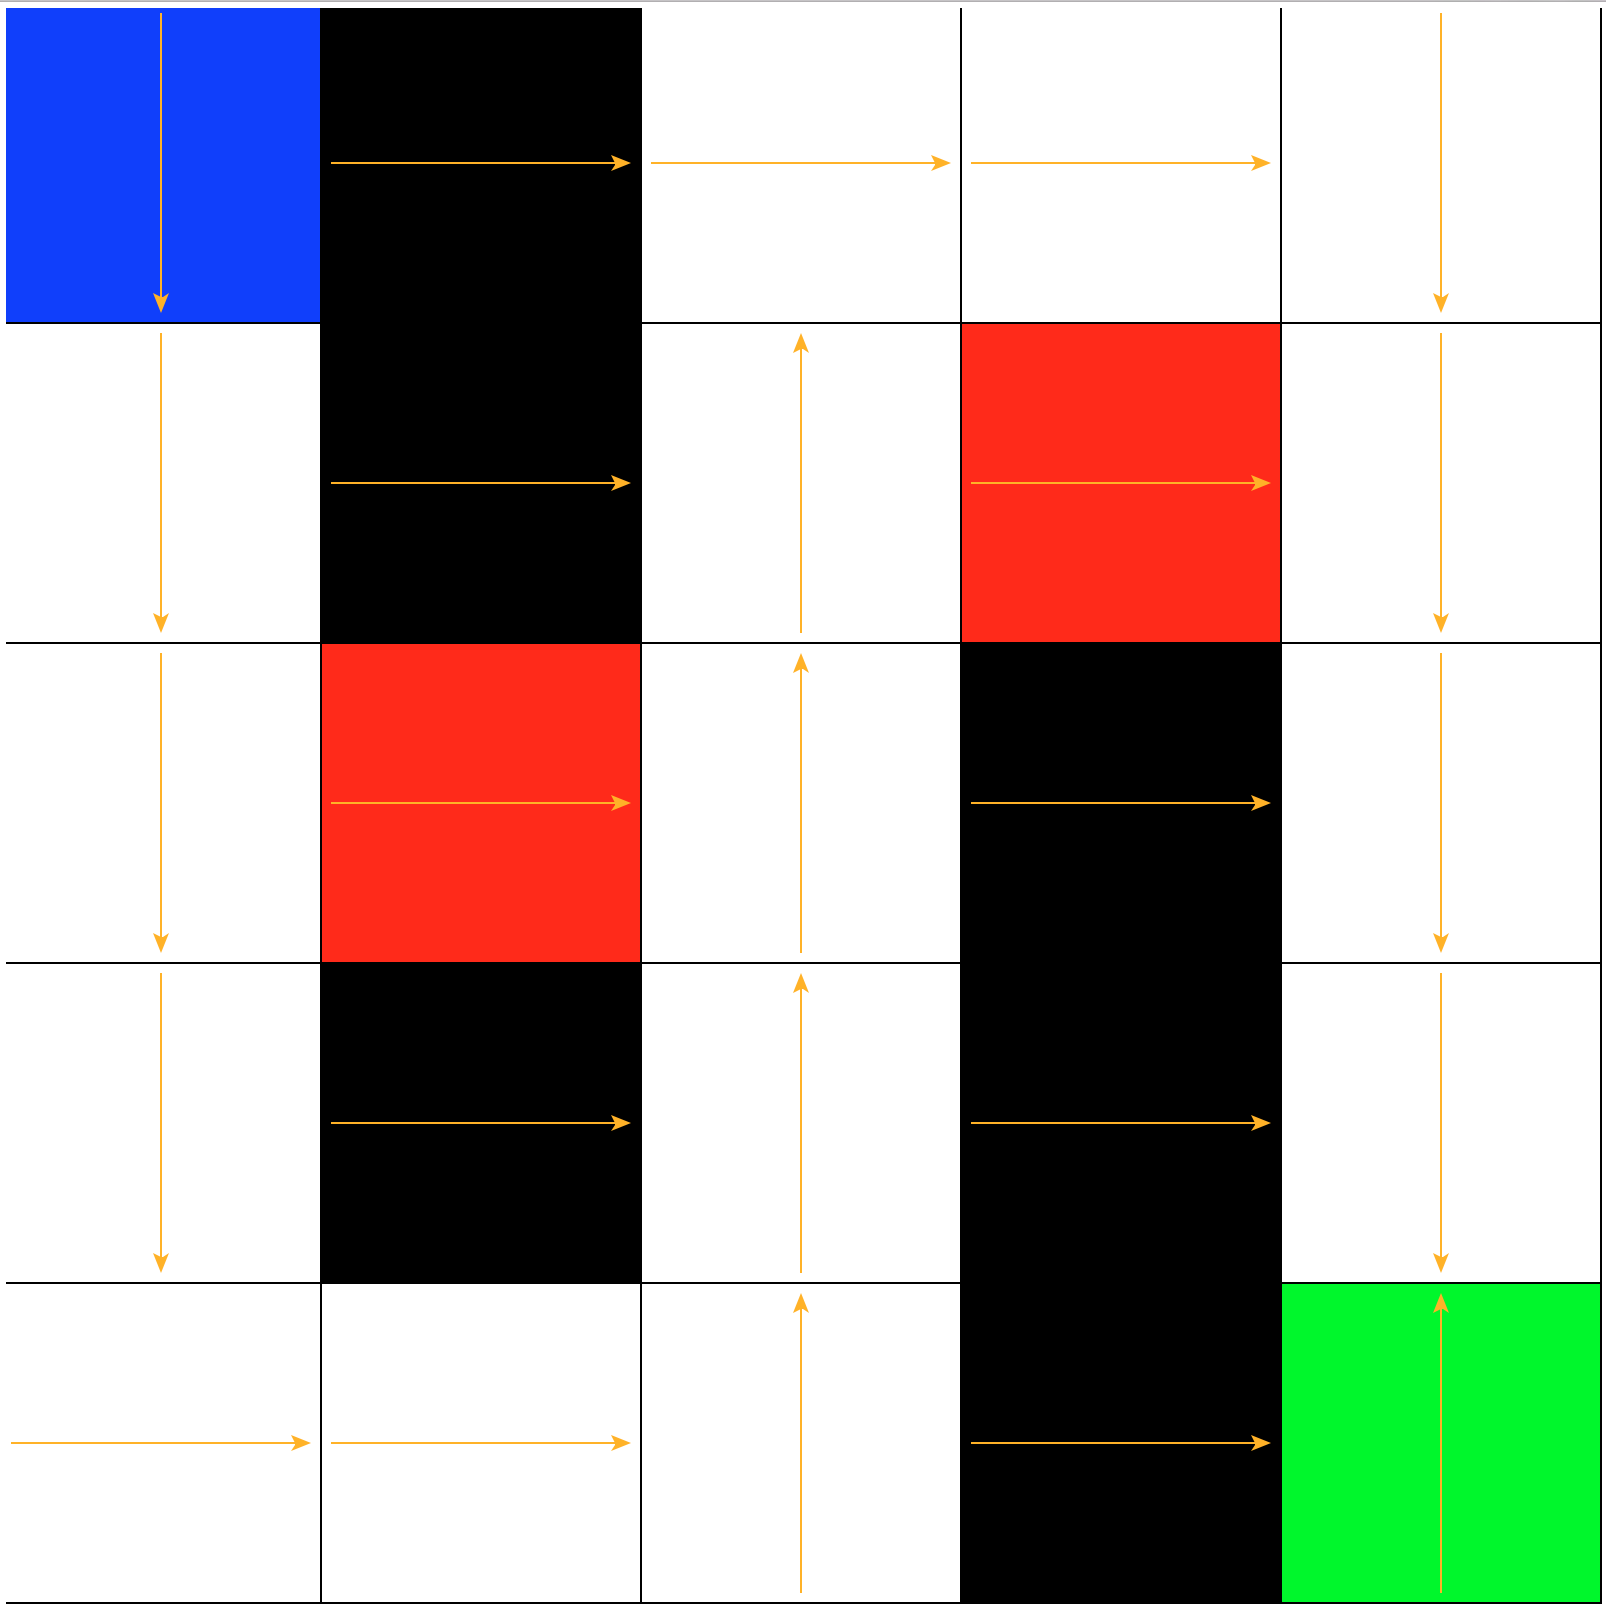
\includegraphics[width=\textwidth]{figures/5x5_viter_r2.png}
                \caption{Reward schema 2\\
                Reward: -5 \\
                Time:  0.0061\\
                Iterations: 81}
                \label{fig:v2}
        \end{subfigure}
        ~ %add desired spacing between images, e. g. ~, \quad, \qquad, \hfill etc.
          %(or a blank line to force the subfigure onto a new line)
        \begin{subfigure}[b]{0.3\textwidth}
                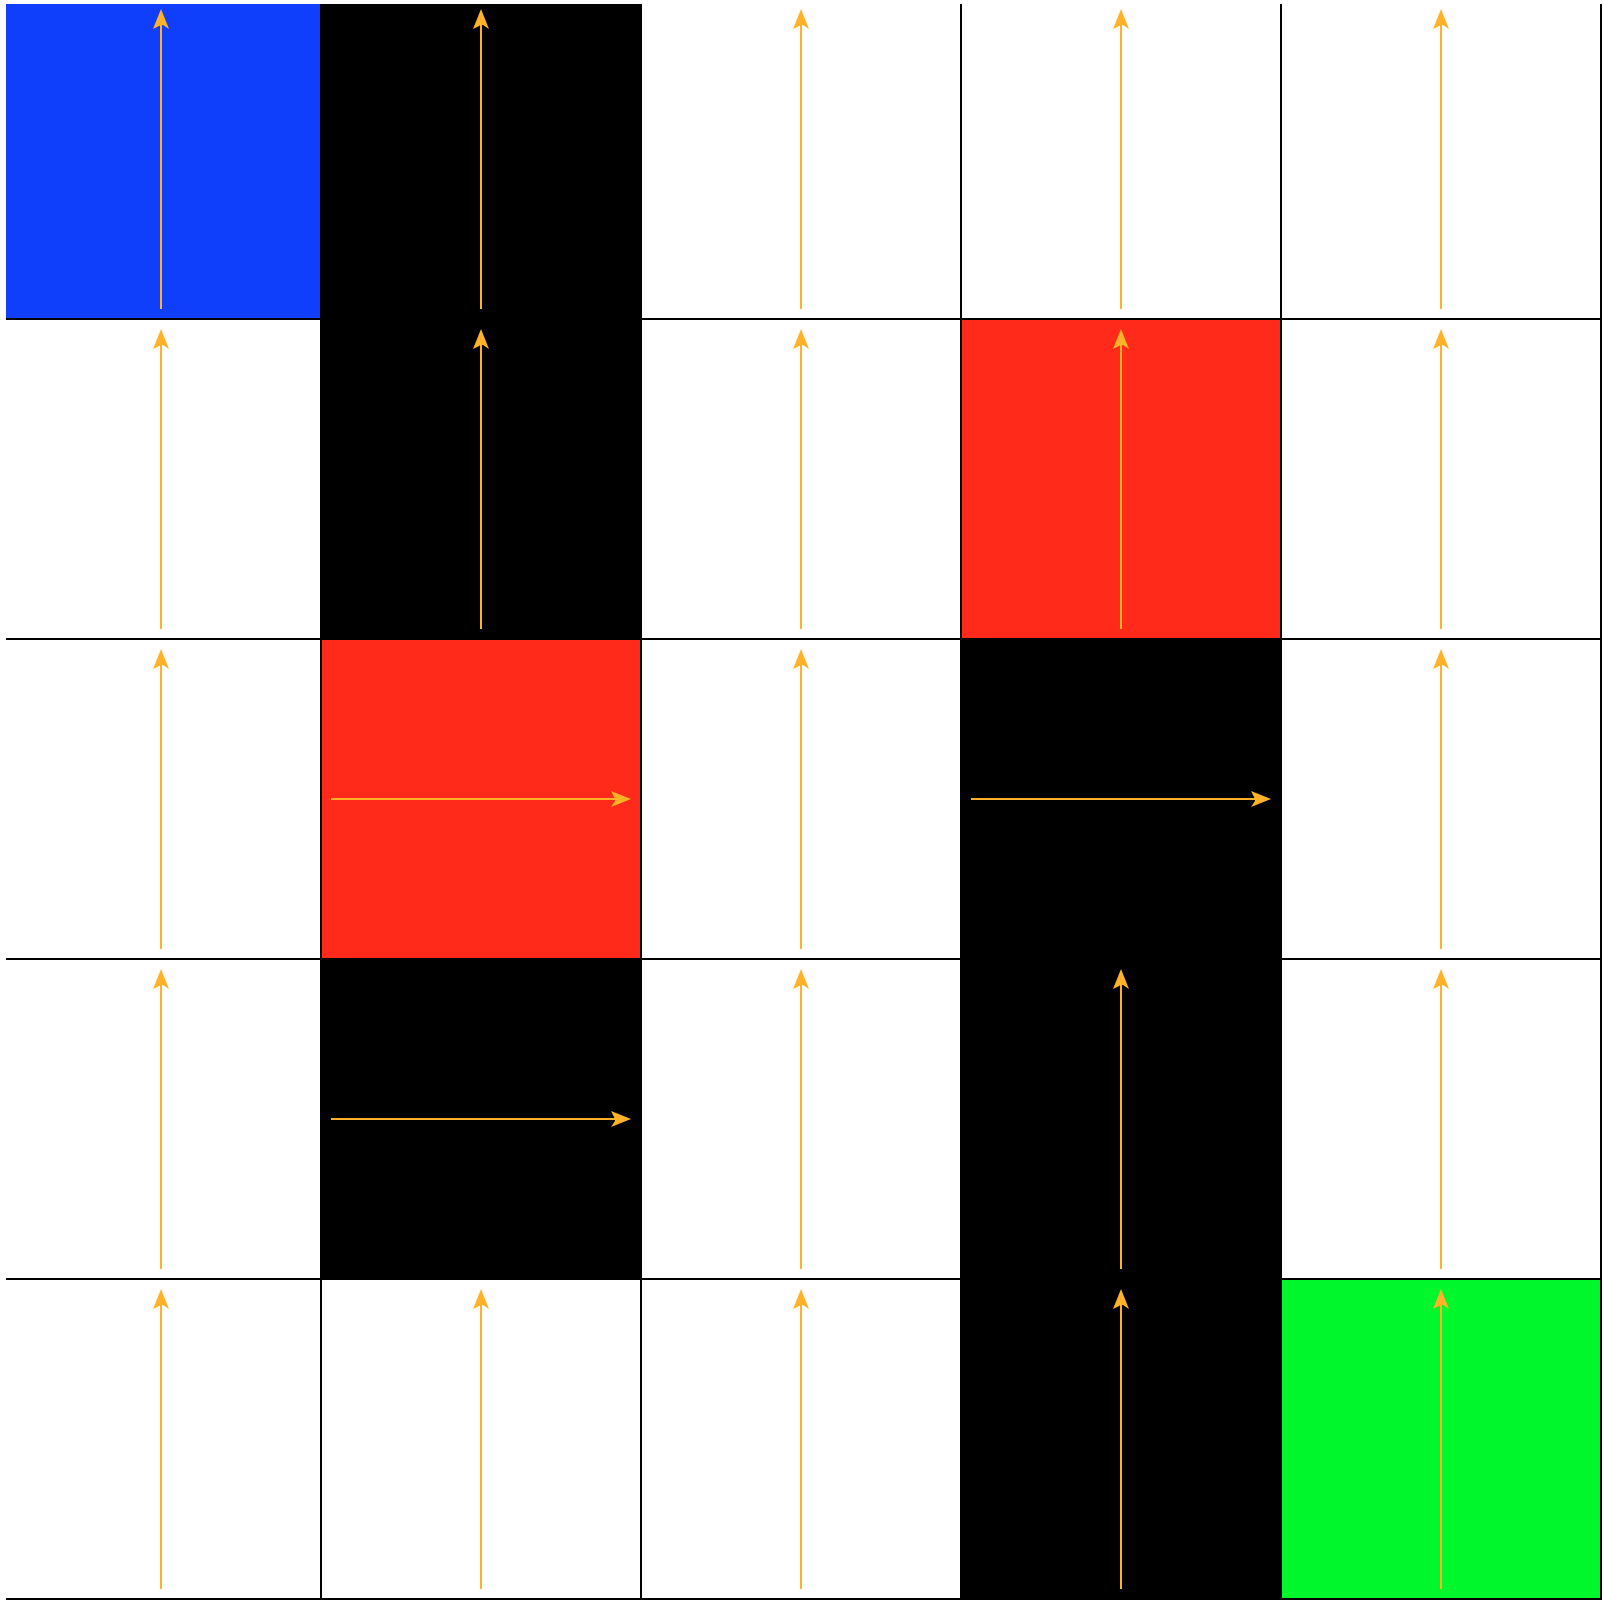
\includegraphics[width=\textwidth]{figures/5x5_viter_r3.png}
                \caption{Reward schema 3\\
                Reward: $\infty$  \\
                Time:  0.0002\\
                Iterations: 2}
                \label{fig:v3}
        \end{subfigure}
        \caption{Policies Learned by Value Iteration}\label{fig:smallval}
\end{figure}
There are some interesting things of note that are happening in value iteration for these simple problems. Firstly in \textit{Figure \ref{fig:v1}} the policy learned was not optimal given the reward structure. For a problem of this size it  possible to trace through by hand and find that the correct policy is the one detailed in \textit{Figure \ref{fig:v2}}. This is most likely an error in the implementation of value iteration.

Another interesting but not surprising result can be seen in  \textit{Figure \ref{fig:v3}}. For this reward schema there is no incentive for the agent to enter the goal but there is an incentive for making arbitrary steps. This causes the agent to try to crash into the upper wall and gain infinite reward.

One further note to make for all subsequent policy figures, the goal state is always terminal though the arrow may suggest otherwise.
\subsubsection{Policy Iteration}
\begin{figure}[H]
        \centering
        \begin{subfigure}[b]{0.3\textwidth}
                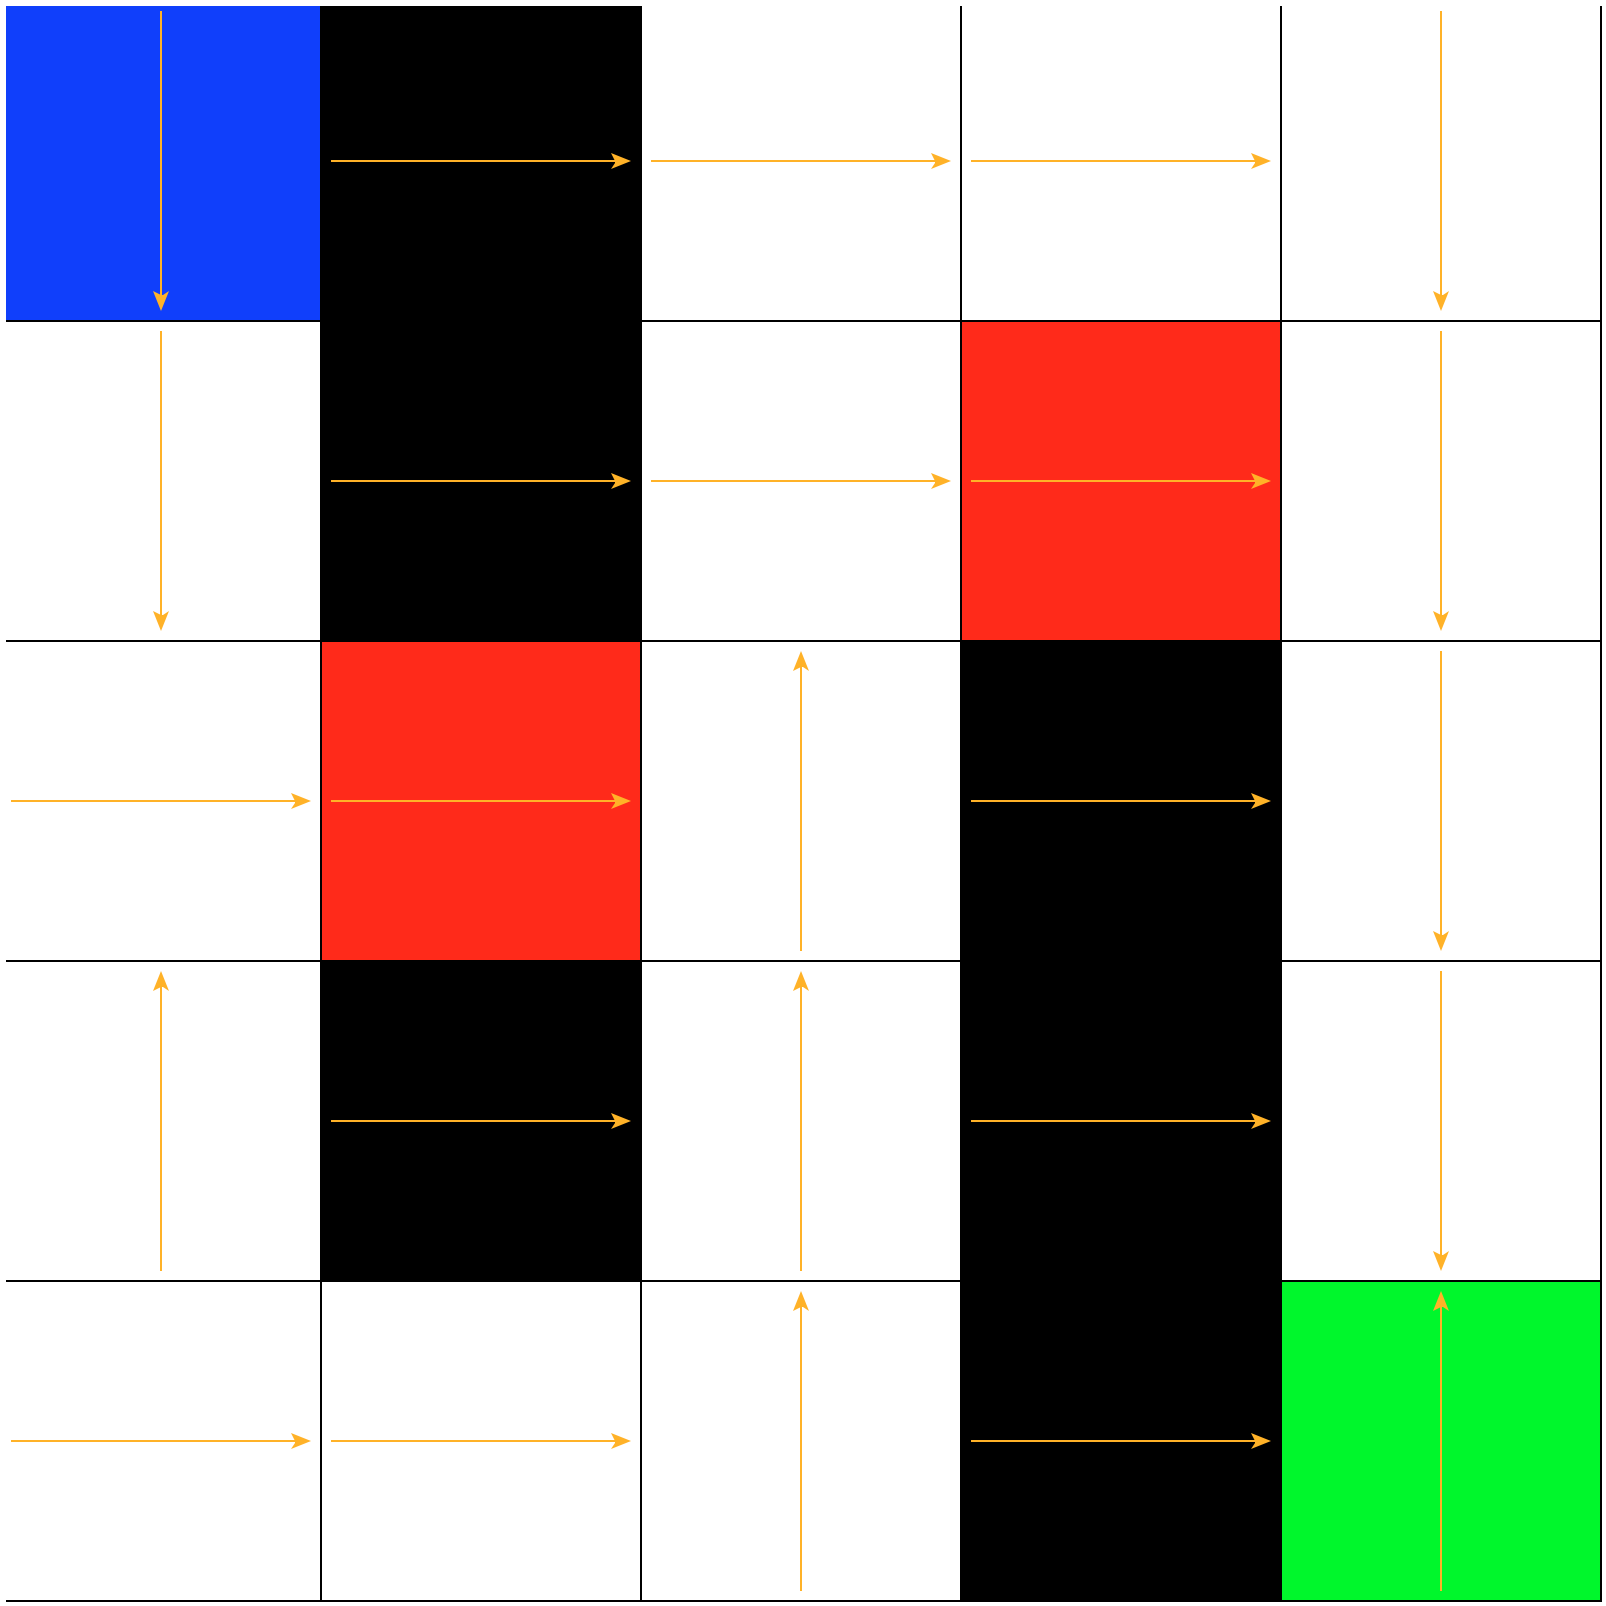
\includegraphics[width=\textwidth]{figures/5x5_piter_r1.png}
                \caption{Reward schema 1\\
                Reward:  7.65 \\
                Time:  0.0094\\
                Iterations: 10 }
                \label{fig:p1}
        \end{subfigure}%
        ~ %add desired spacing between images, e. g. ~, \quad, \qquad, \hfill etc.
          %(or a blank line to force the subfigure onto a new line)
        \begin{subfigure}[b]{0.3\textwidth}
                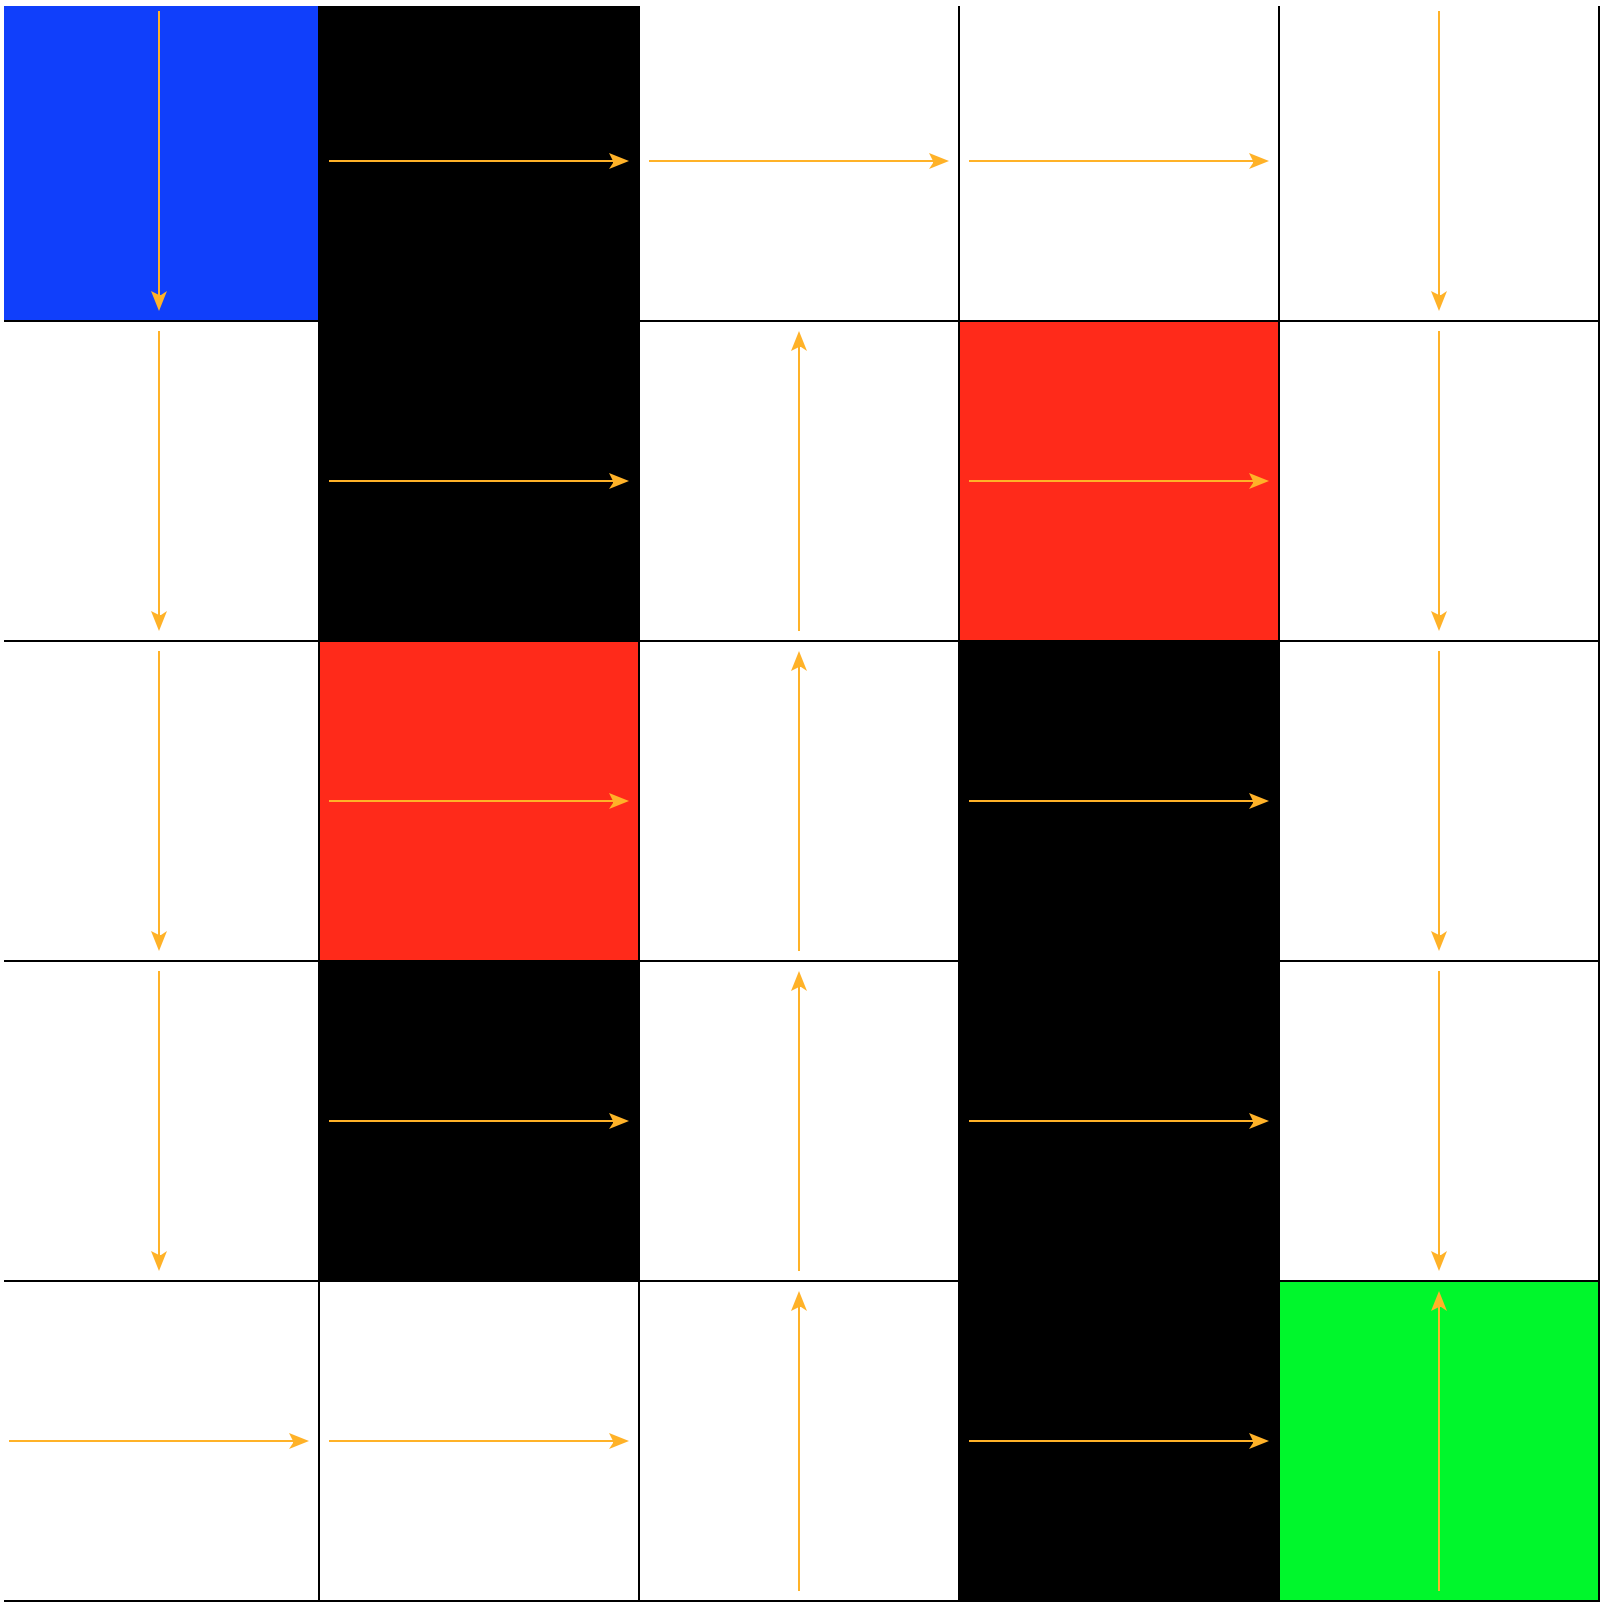
\includegraphics[width=\textwidth]{figures/5x5_piter_r2.png}
                \caption{Reward schema 2\\
                Reward: -5 \\
                Time:  0.0112\\
                Iterations: 11 }
                \label{fig:p2}
        \end{subfigure}
        ~ %add desired spacing between images, e. g. ~, \quad, \qquad, \hfill etc.
          %(or a blank line to force the subfigure onto a new line)
        \begin{subfigure}[b]{0.3\textwidth}
                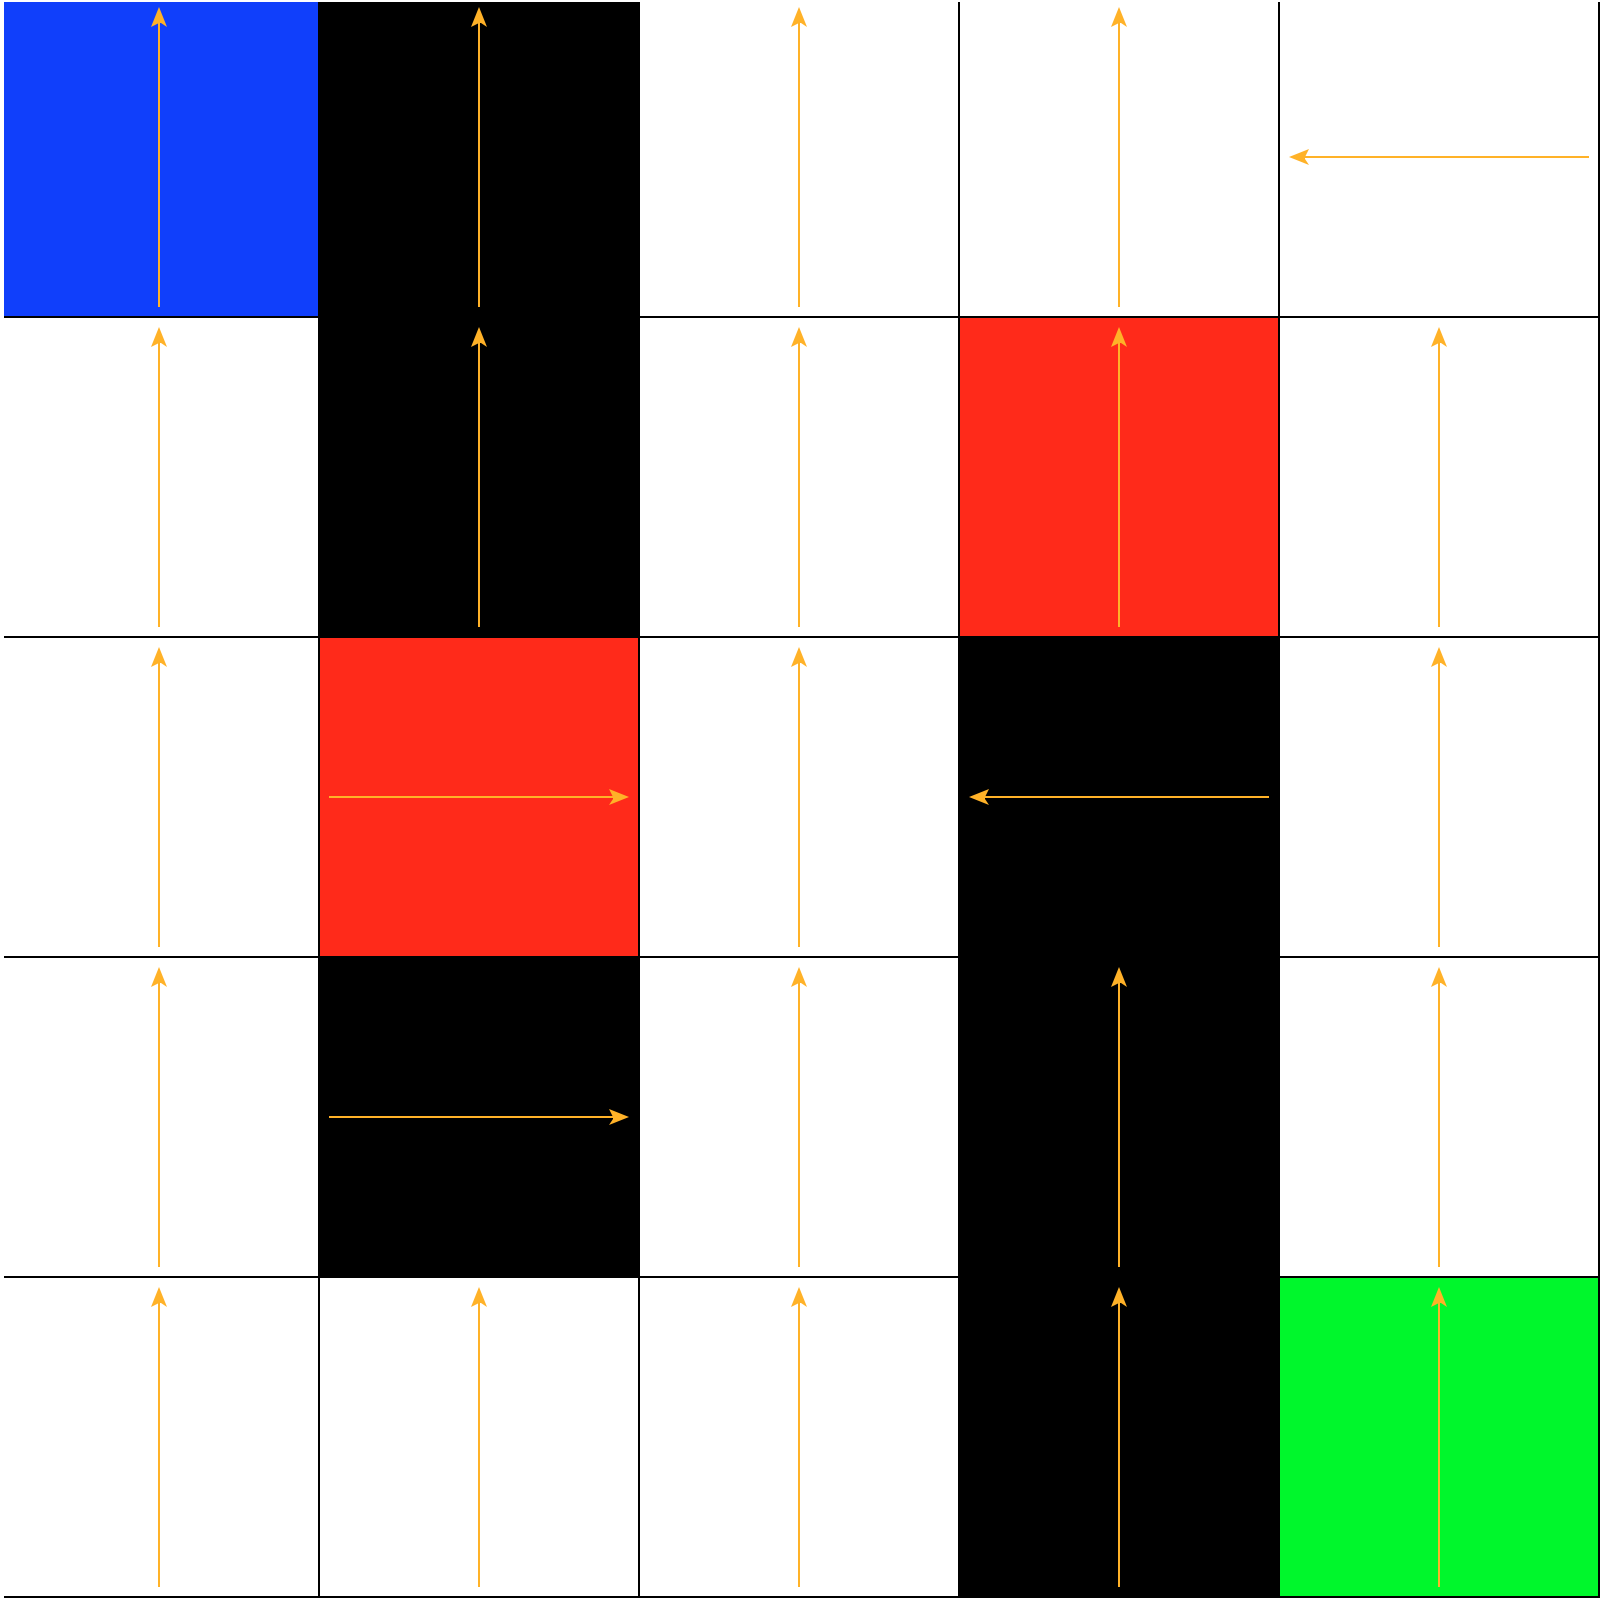
\includegraphics[width=\textwidth]{figures/5x5_piter_r3.png}
                \caption{Reward schema 3\\
                Reward: $\infty$ \\
                Time: 0.5076\\
                Iterations: 1000 (max)}
                \label{fig:p3}
        \end{subfigure}
        \caption{Policies Learned by Policy Iteration}\label{fig:animals}
\end{figure}
Policy iteration demonstrates the same results as \textit{Figure \ref{fig:smallval}}. Again, this is most likely due to the implementation.

As expected policy iteration takes fewer iterations than value iteration (except in \textit{Figure \ref{fig:p3}}). It does take slightly longer in all cases to find what it believes to be the optimal policy. This would suggest that policy iteration has more computationally costly iterations, but does fewer of them overall. \textit{Figure \ref{fig:p3}} is an exceptional case since there is no optimal policy that causes the MDP to achieve a terminal state.

\subsubsection{Q-Learning}
\begin{figure}[H]
        \centering
        \begin{subfigure}[b]{0.3\textwidth}
                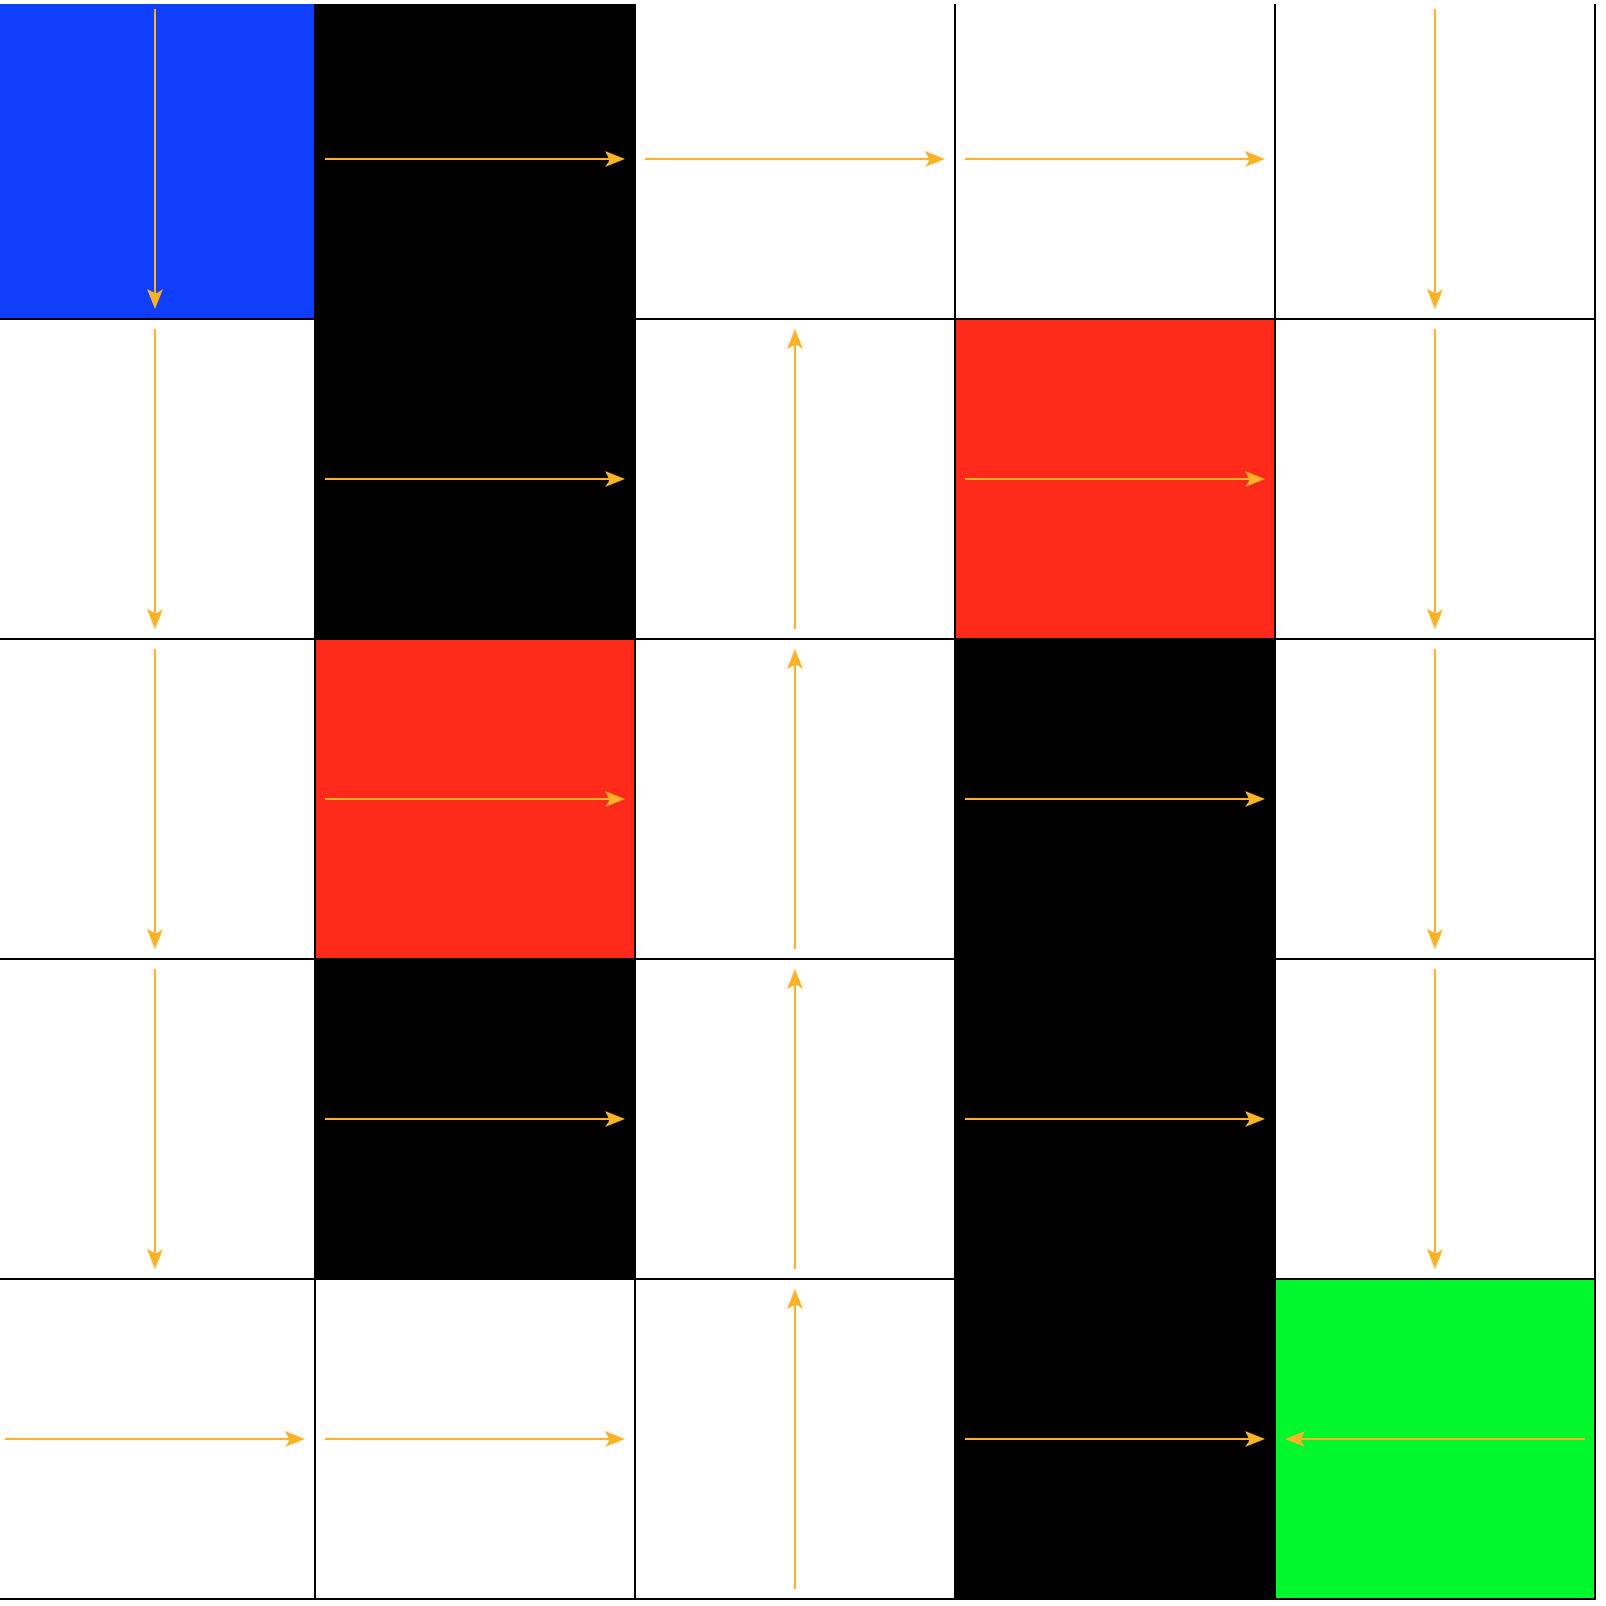
\includegraphics[width=\textwidth]{figures/5x5_qlearn_r1.png}
                \caption{Reward schema 1\\ 
                Reward:  9.25 \\
                Time:  1.353 \\
                Iterations:  25013 }
                \label{fig:q1}
        \end{subfigure}%
        ~ %add desired spacing between images, e. g. ~, \quad, \qquad, \hfill etc.
          %(or a blank line to force the subfigure onto a new line)
        \begin{subfigure}[b]{0.3\textwidth}
                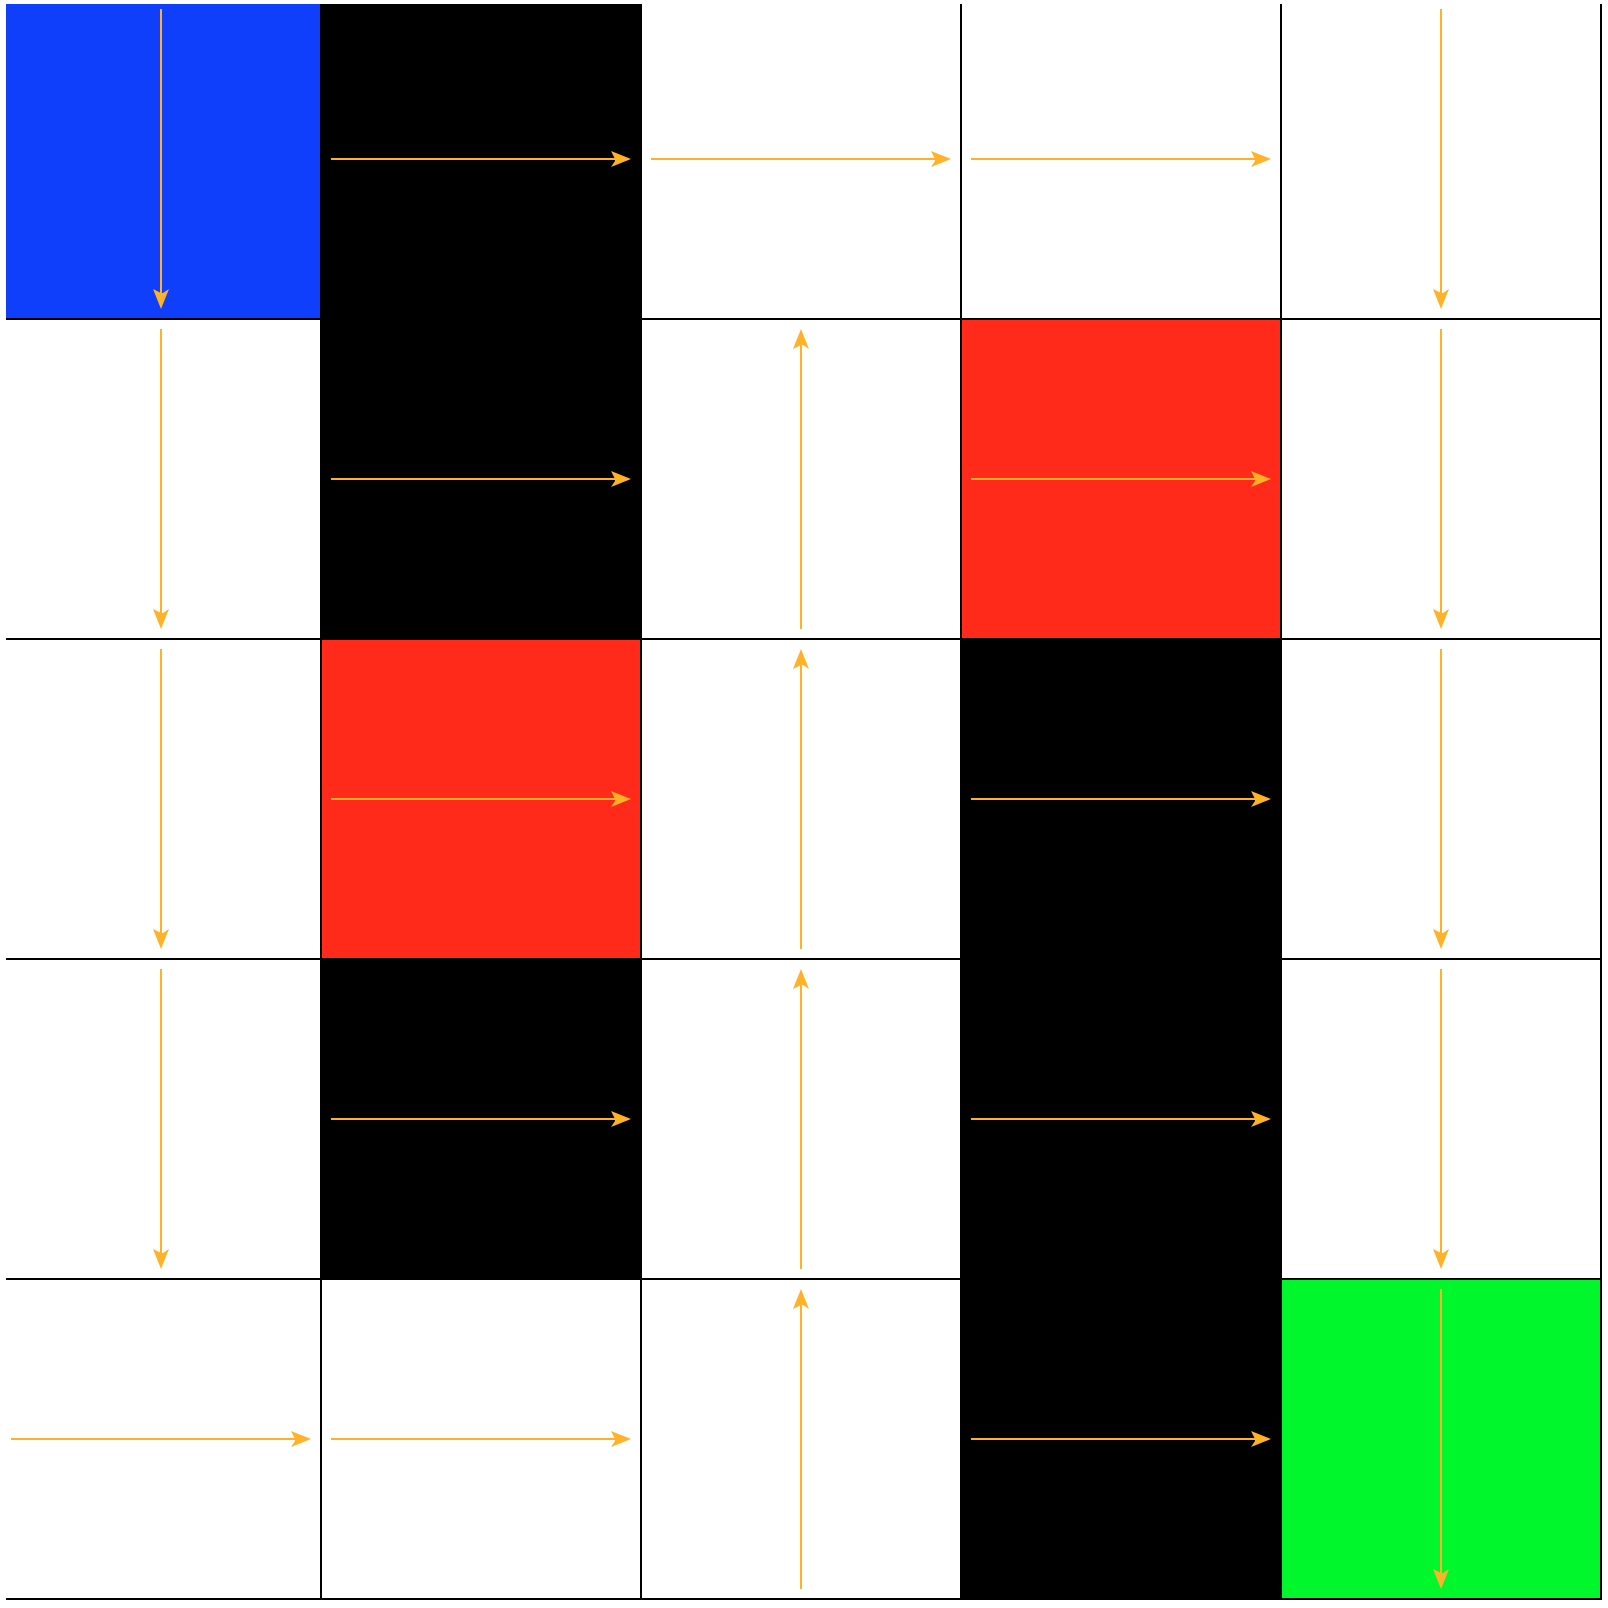
\includegraphics[width=\textwidth]{figures/5x5_qlearn_r2.png}
                \caption{Reward schema 2\\
                Reward: -5\\
                Time:  1.340\\
                Iterations: 25597 }
                \label{fig:q2}
        \end{subfigure}
        ~ %add desired spacing between images, e. g. ~, \quad, \qquad, \hfill etc.
          %(or a blank line to force the subfigure onto a new line)
        \begin{subfigure}[b]{0.3\textwidth}
                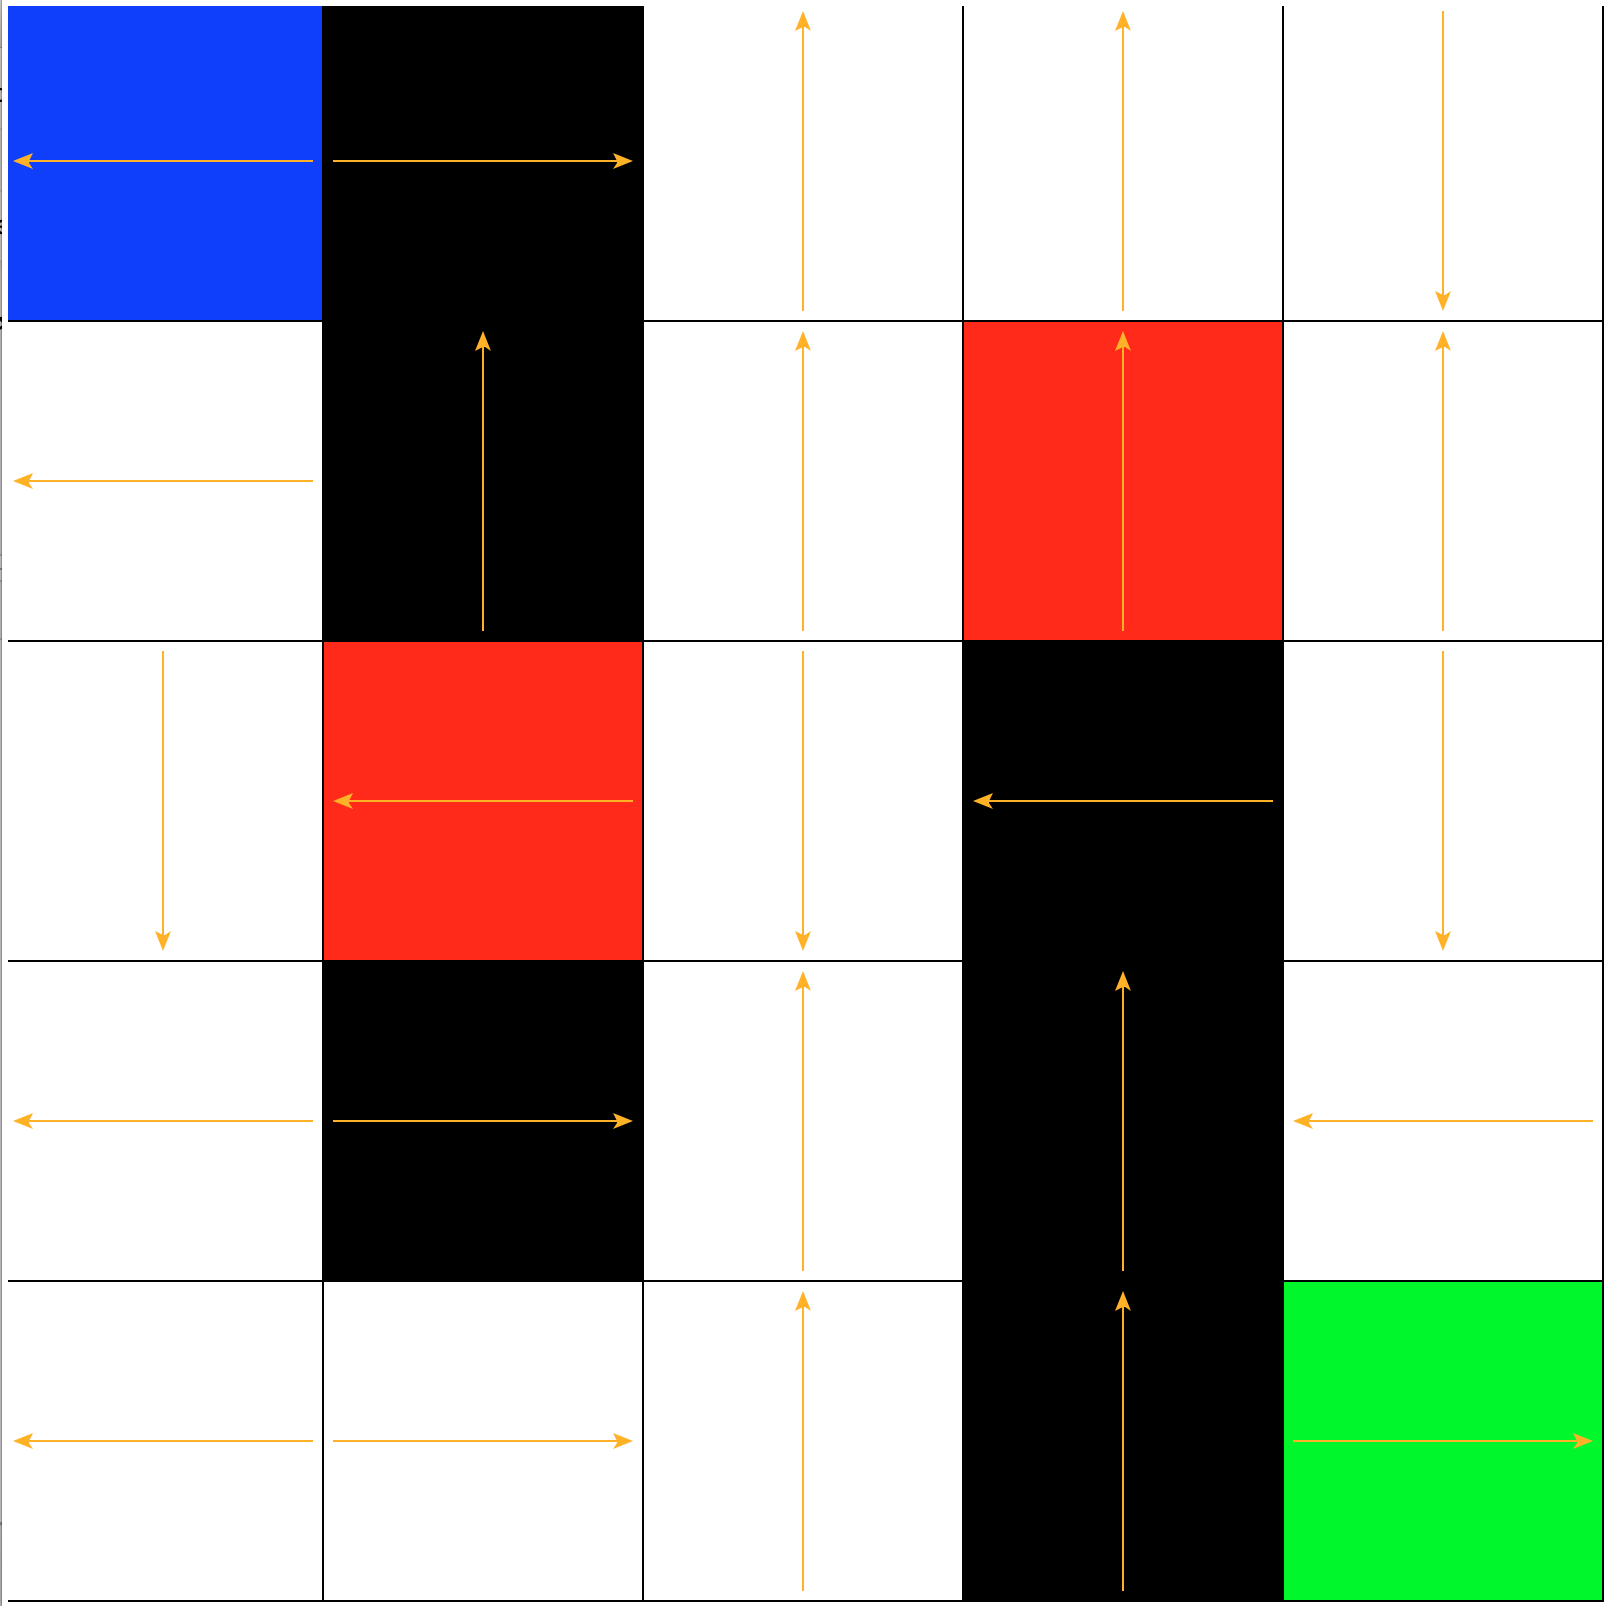
\includegraphics[width=\textwidth]{figures/5x5_qlearn_r3.png}
                \caption{Reward schema 3 \\
                Reward: $\infty$\\
                Time: 1.677 \\
                Iterations: 65465 }
                \label{fig:q3}
        \end{subfigure}
        \caption{Policies Learned by Q-Learning}\label{fig:animals}
\end{figure}

The implementation of Q-Learning is completely separate from the implementations of both policy and value iteration, so it is not running into the same pitfalls as either of those algorithms. The number of iterations for Q-Learning is much higher than either of the other techniques. This is to be expected from the implementation of the algorithm. The number of episodes has been set to to run a minimum of 1000 times and each episode will iterate over each state at least 1 time. This leads to a minimum number of iterations of $25000$. This number of episodes was chosen to increase liklihood of convergence for large MDP problems. It could be liberally adjusted to improve performance for smaller problems.
\subsection{50x50 World}

The reward schema for the larger gridworld is modified to take into account the large number of steps that are needed to make it to the goal. 

\begin{enumerate}
\item Goal State: +1000; Step Penalty: -0.05; Penalty State: -3;
\item Goal State: +1000; Step Penalty: -5: Penalty State: -20;
\item Goal State: 0; Step Penalty: 1; Penalty State: -2;
\end{enumerate}

\subsubsection{Value Iteration}
\begin{figure}[H]
        \centering
        \begin{subfigure}[b]{0.3\textwidth}
                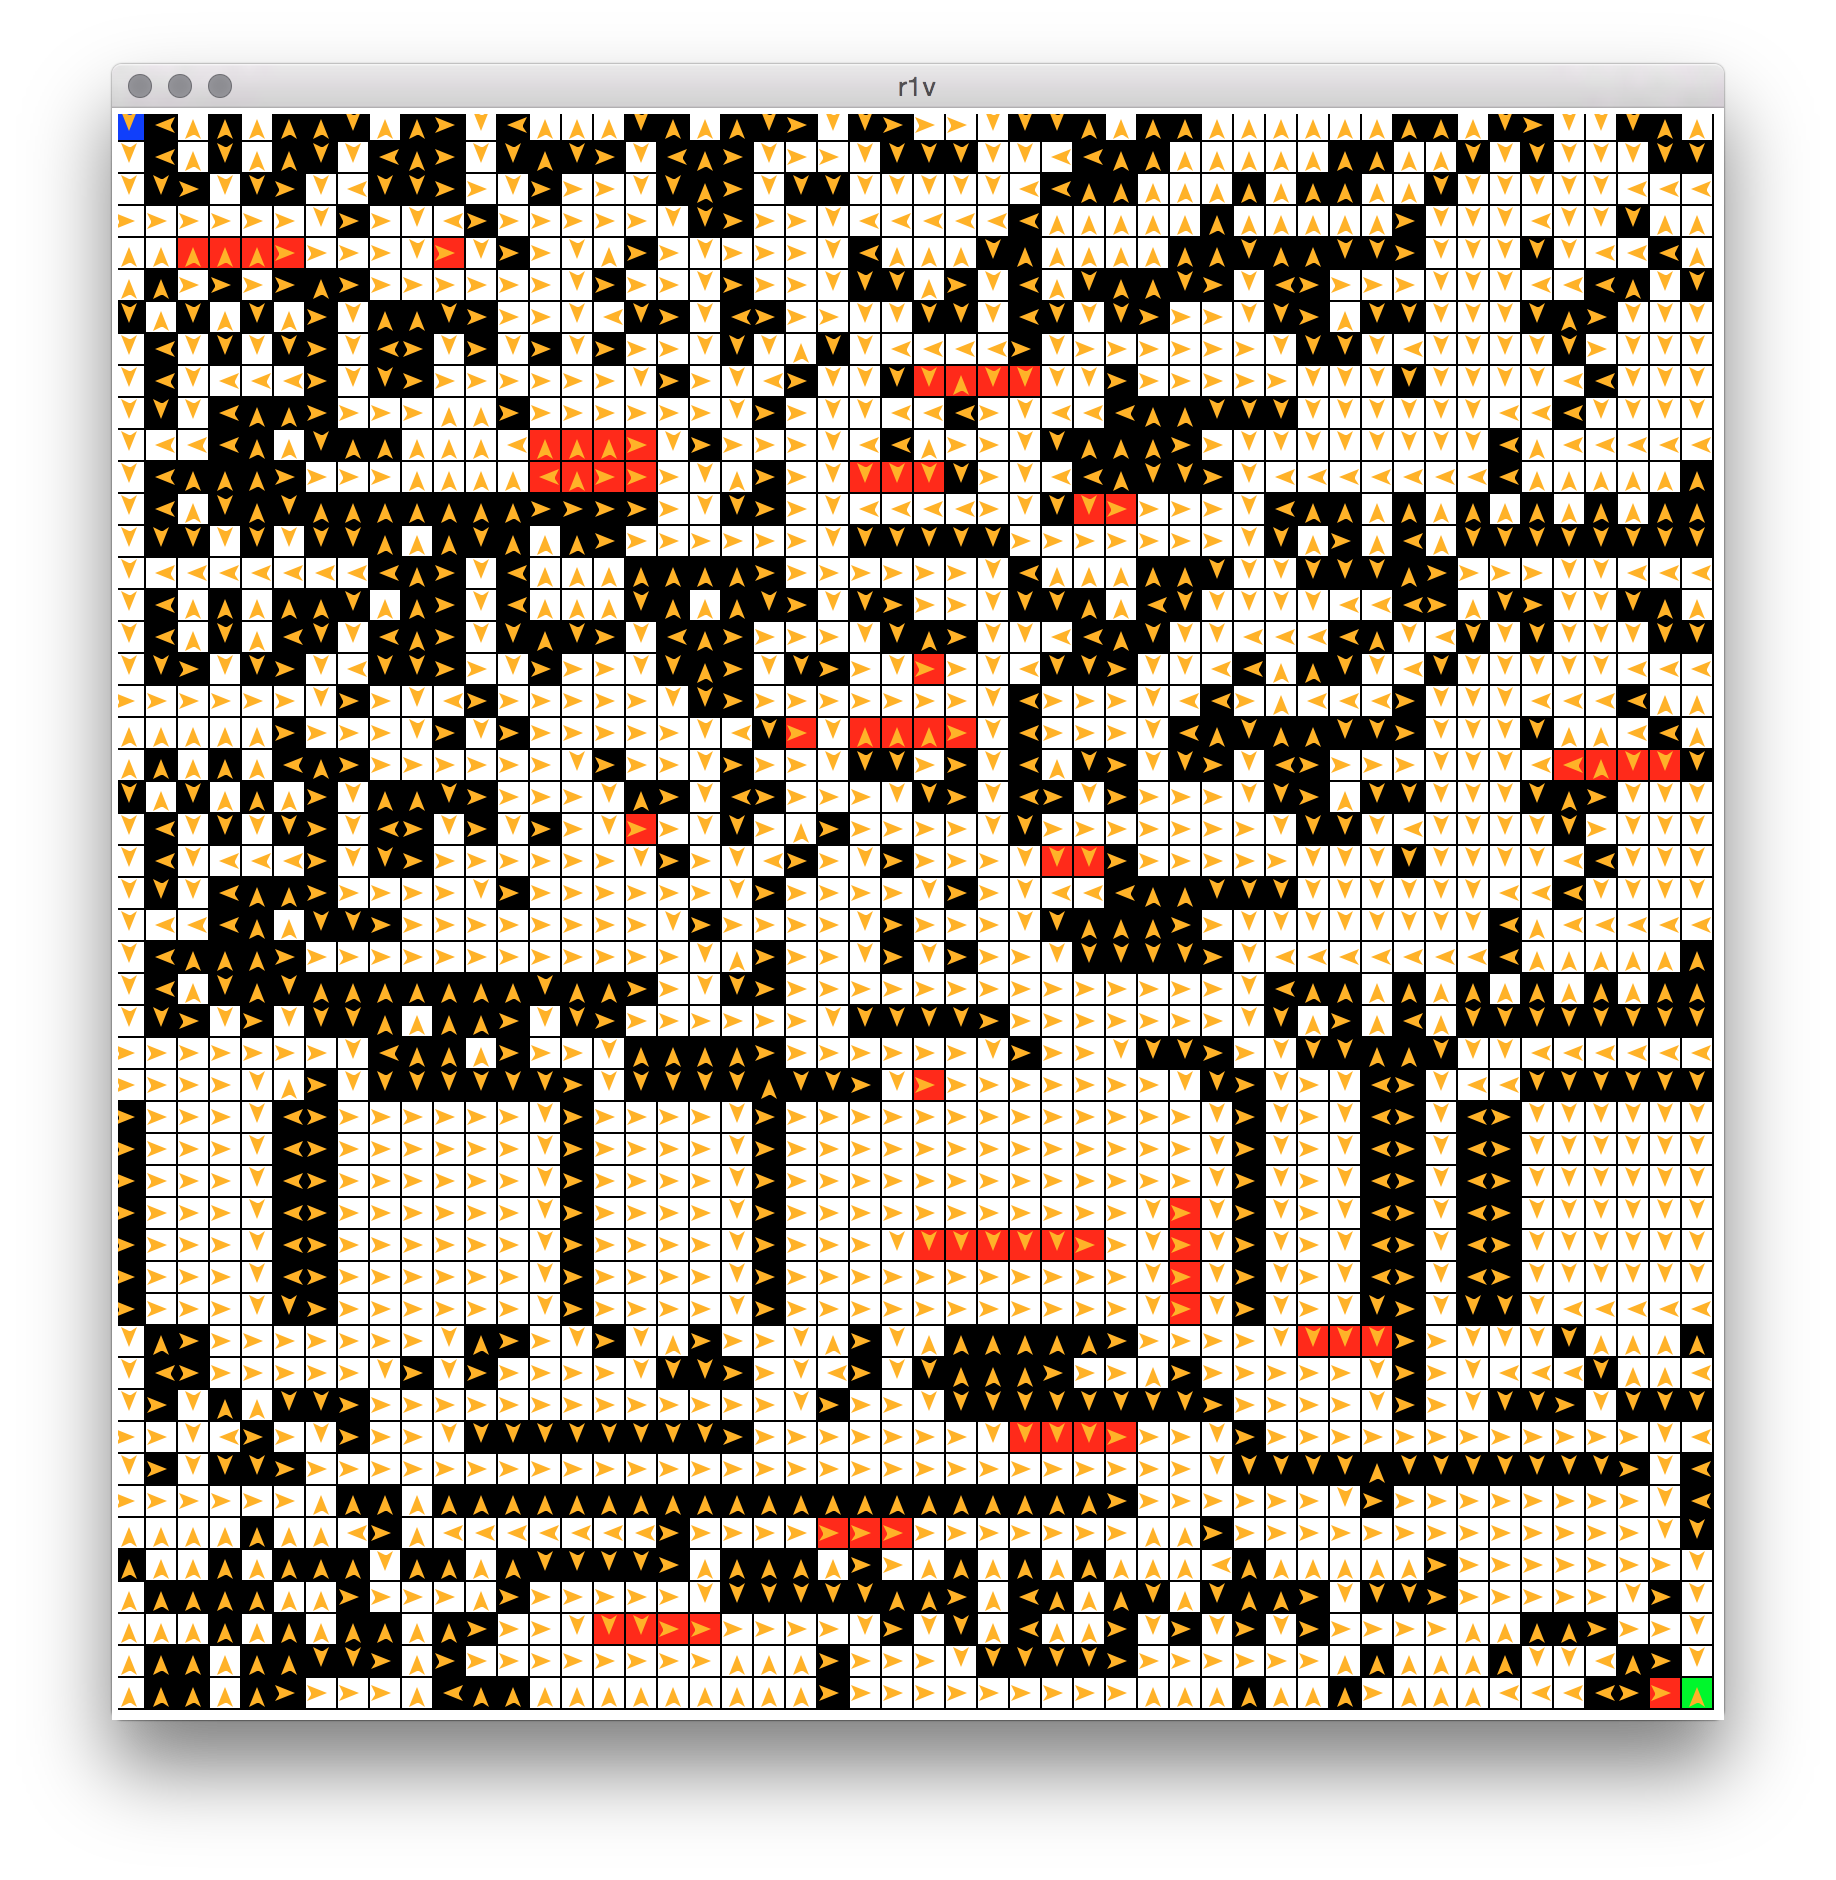
\includegraphics[width=\textwidth]{figures/50x50_v_r1.png}
                \caption{Reward schema 1\\
                Reward:  995.15\\
                Time:  1.5505\\
                Iterations: 131}
                \label{fig:gull}
        \end{subfigure}%
        ~ %add desired spacing between images, e. g. ~, \quad, \qquad, \hfill etc.
          %(or a blank line to force the subfigure onto a new line)
        \begin{subfigure}[b]{0.3\textwidth}
                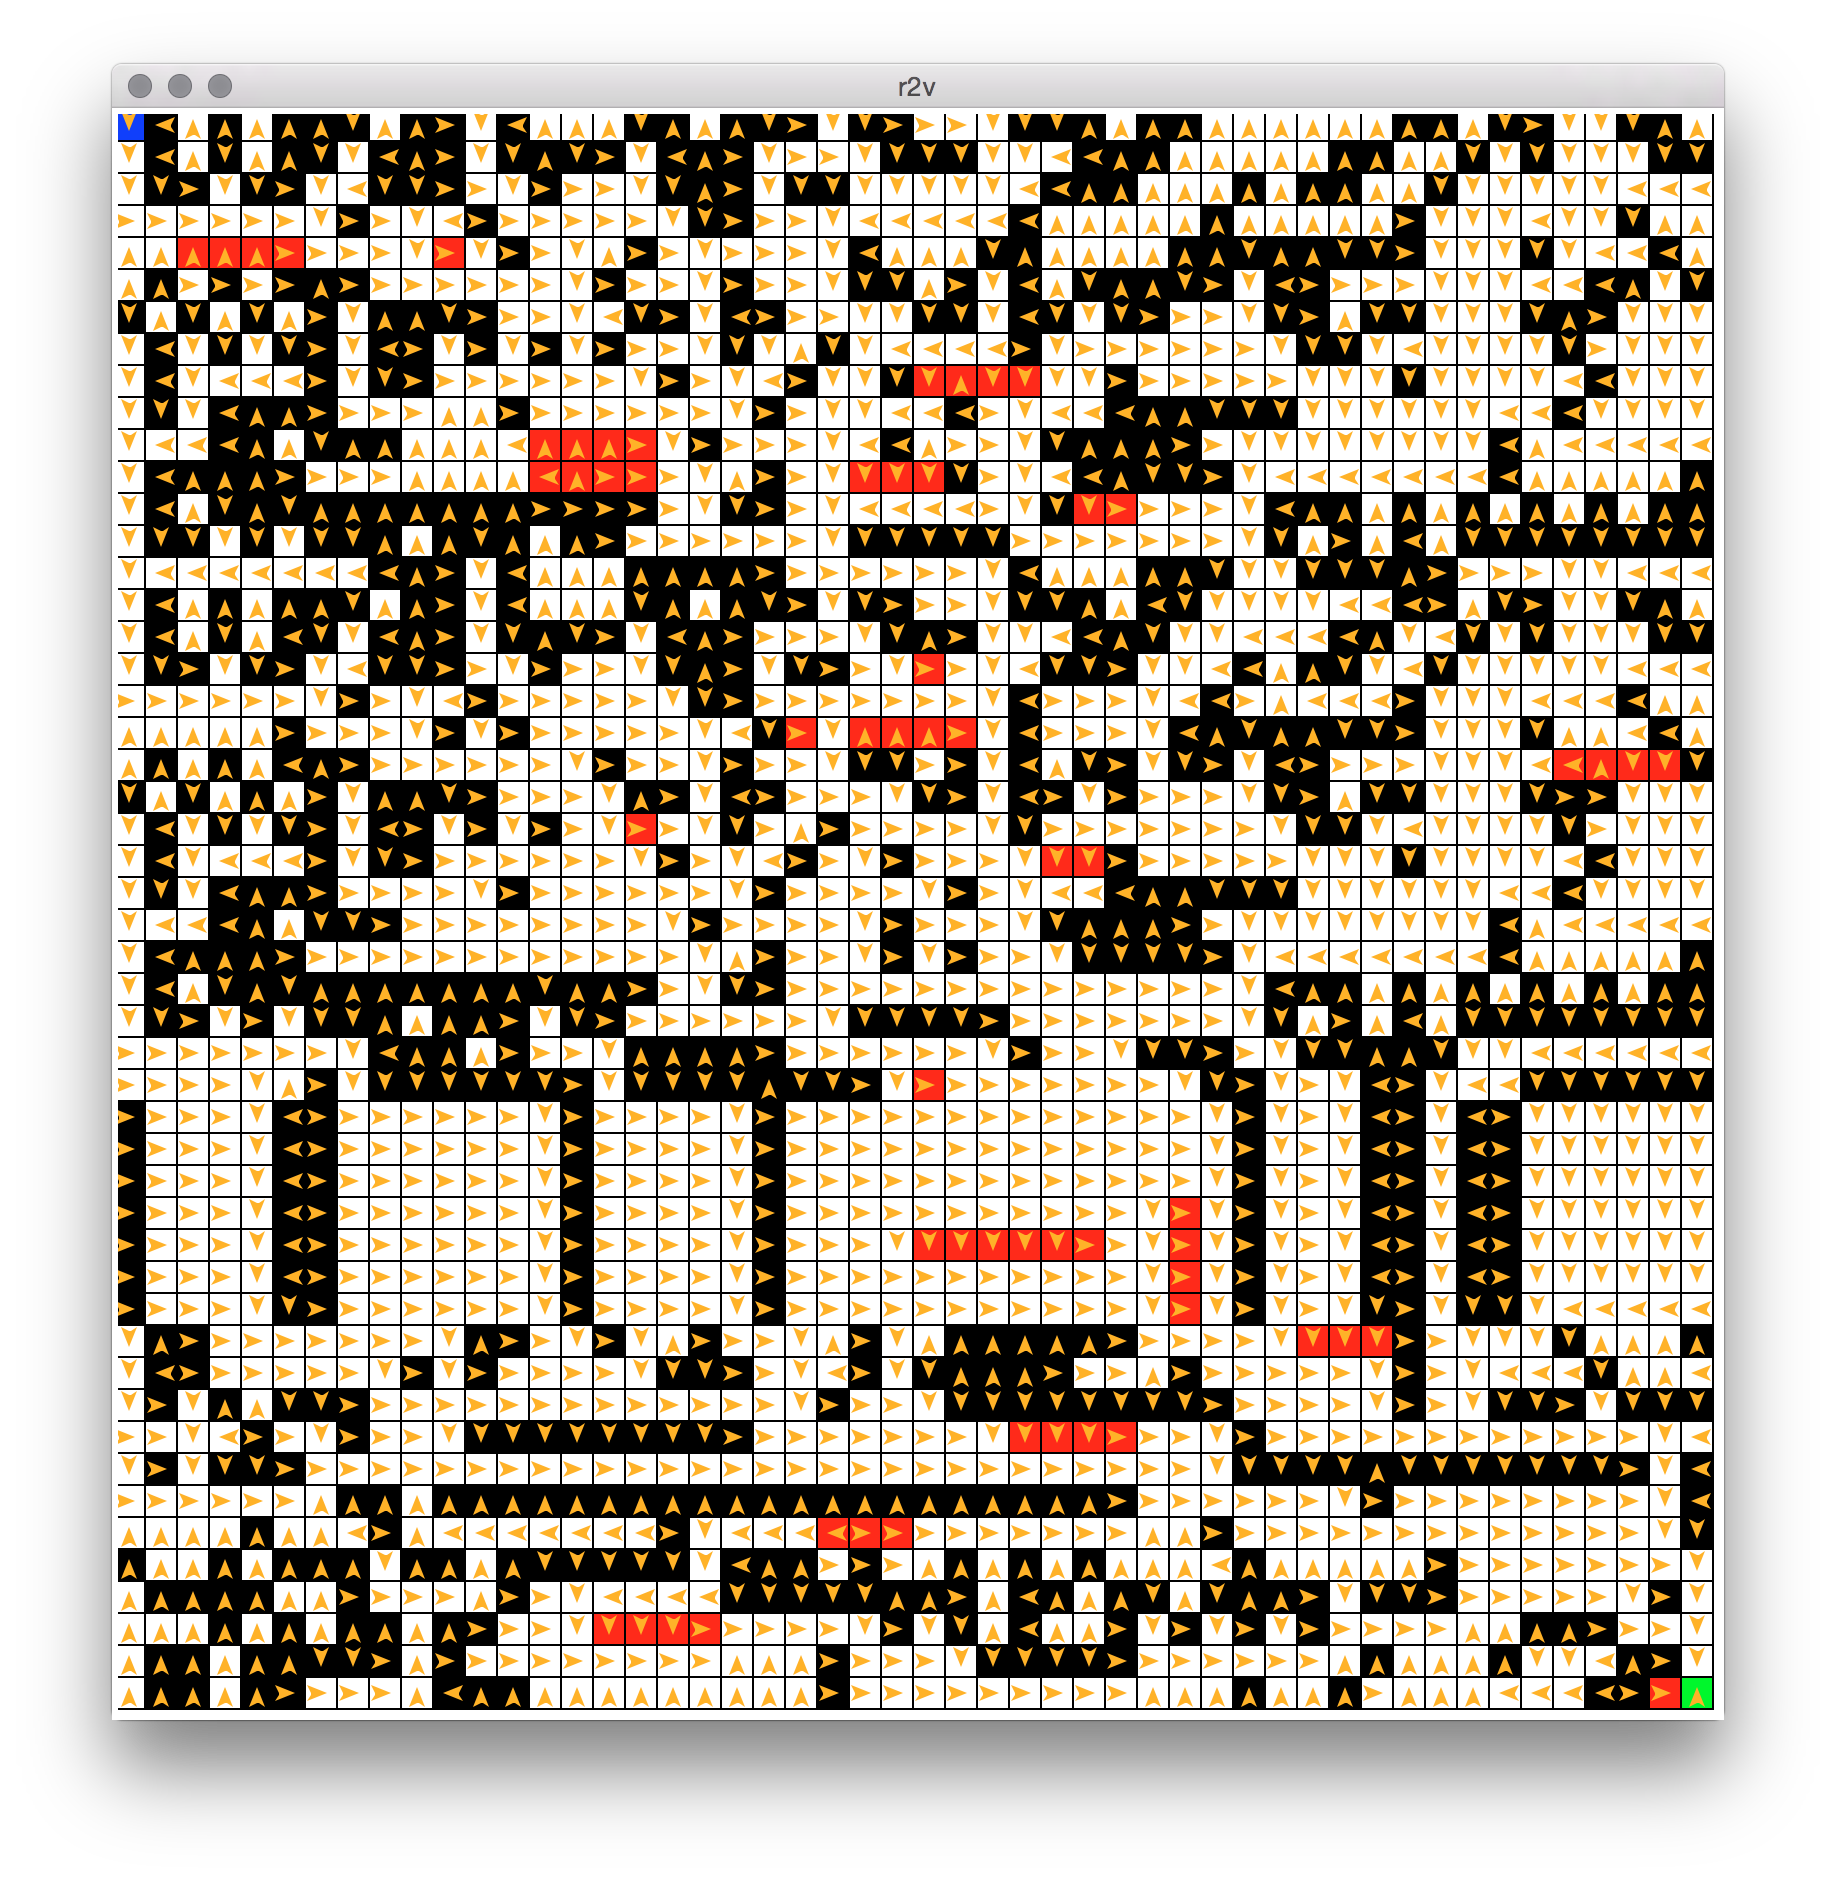
\includegraphics[width=\textwidth]{figures/50x50_v_r2.png}
                \caption{Reward schema 2\\
                Reward: 515 \\
                Time:  1.6819\\
                Iterations: 131}
                \label{fig:tiger}
        \end{subfigure}
        ~ %add desired spacing between images, e. g. ~, \quad, \qquad, \hfill etc.
          %(or a blank line to force the subfigure onto a new line)
        \begin{subfigure}[b]{0.3\textwidth}
                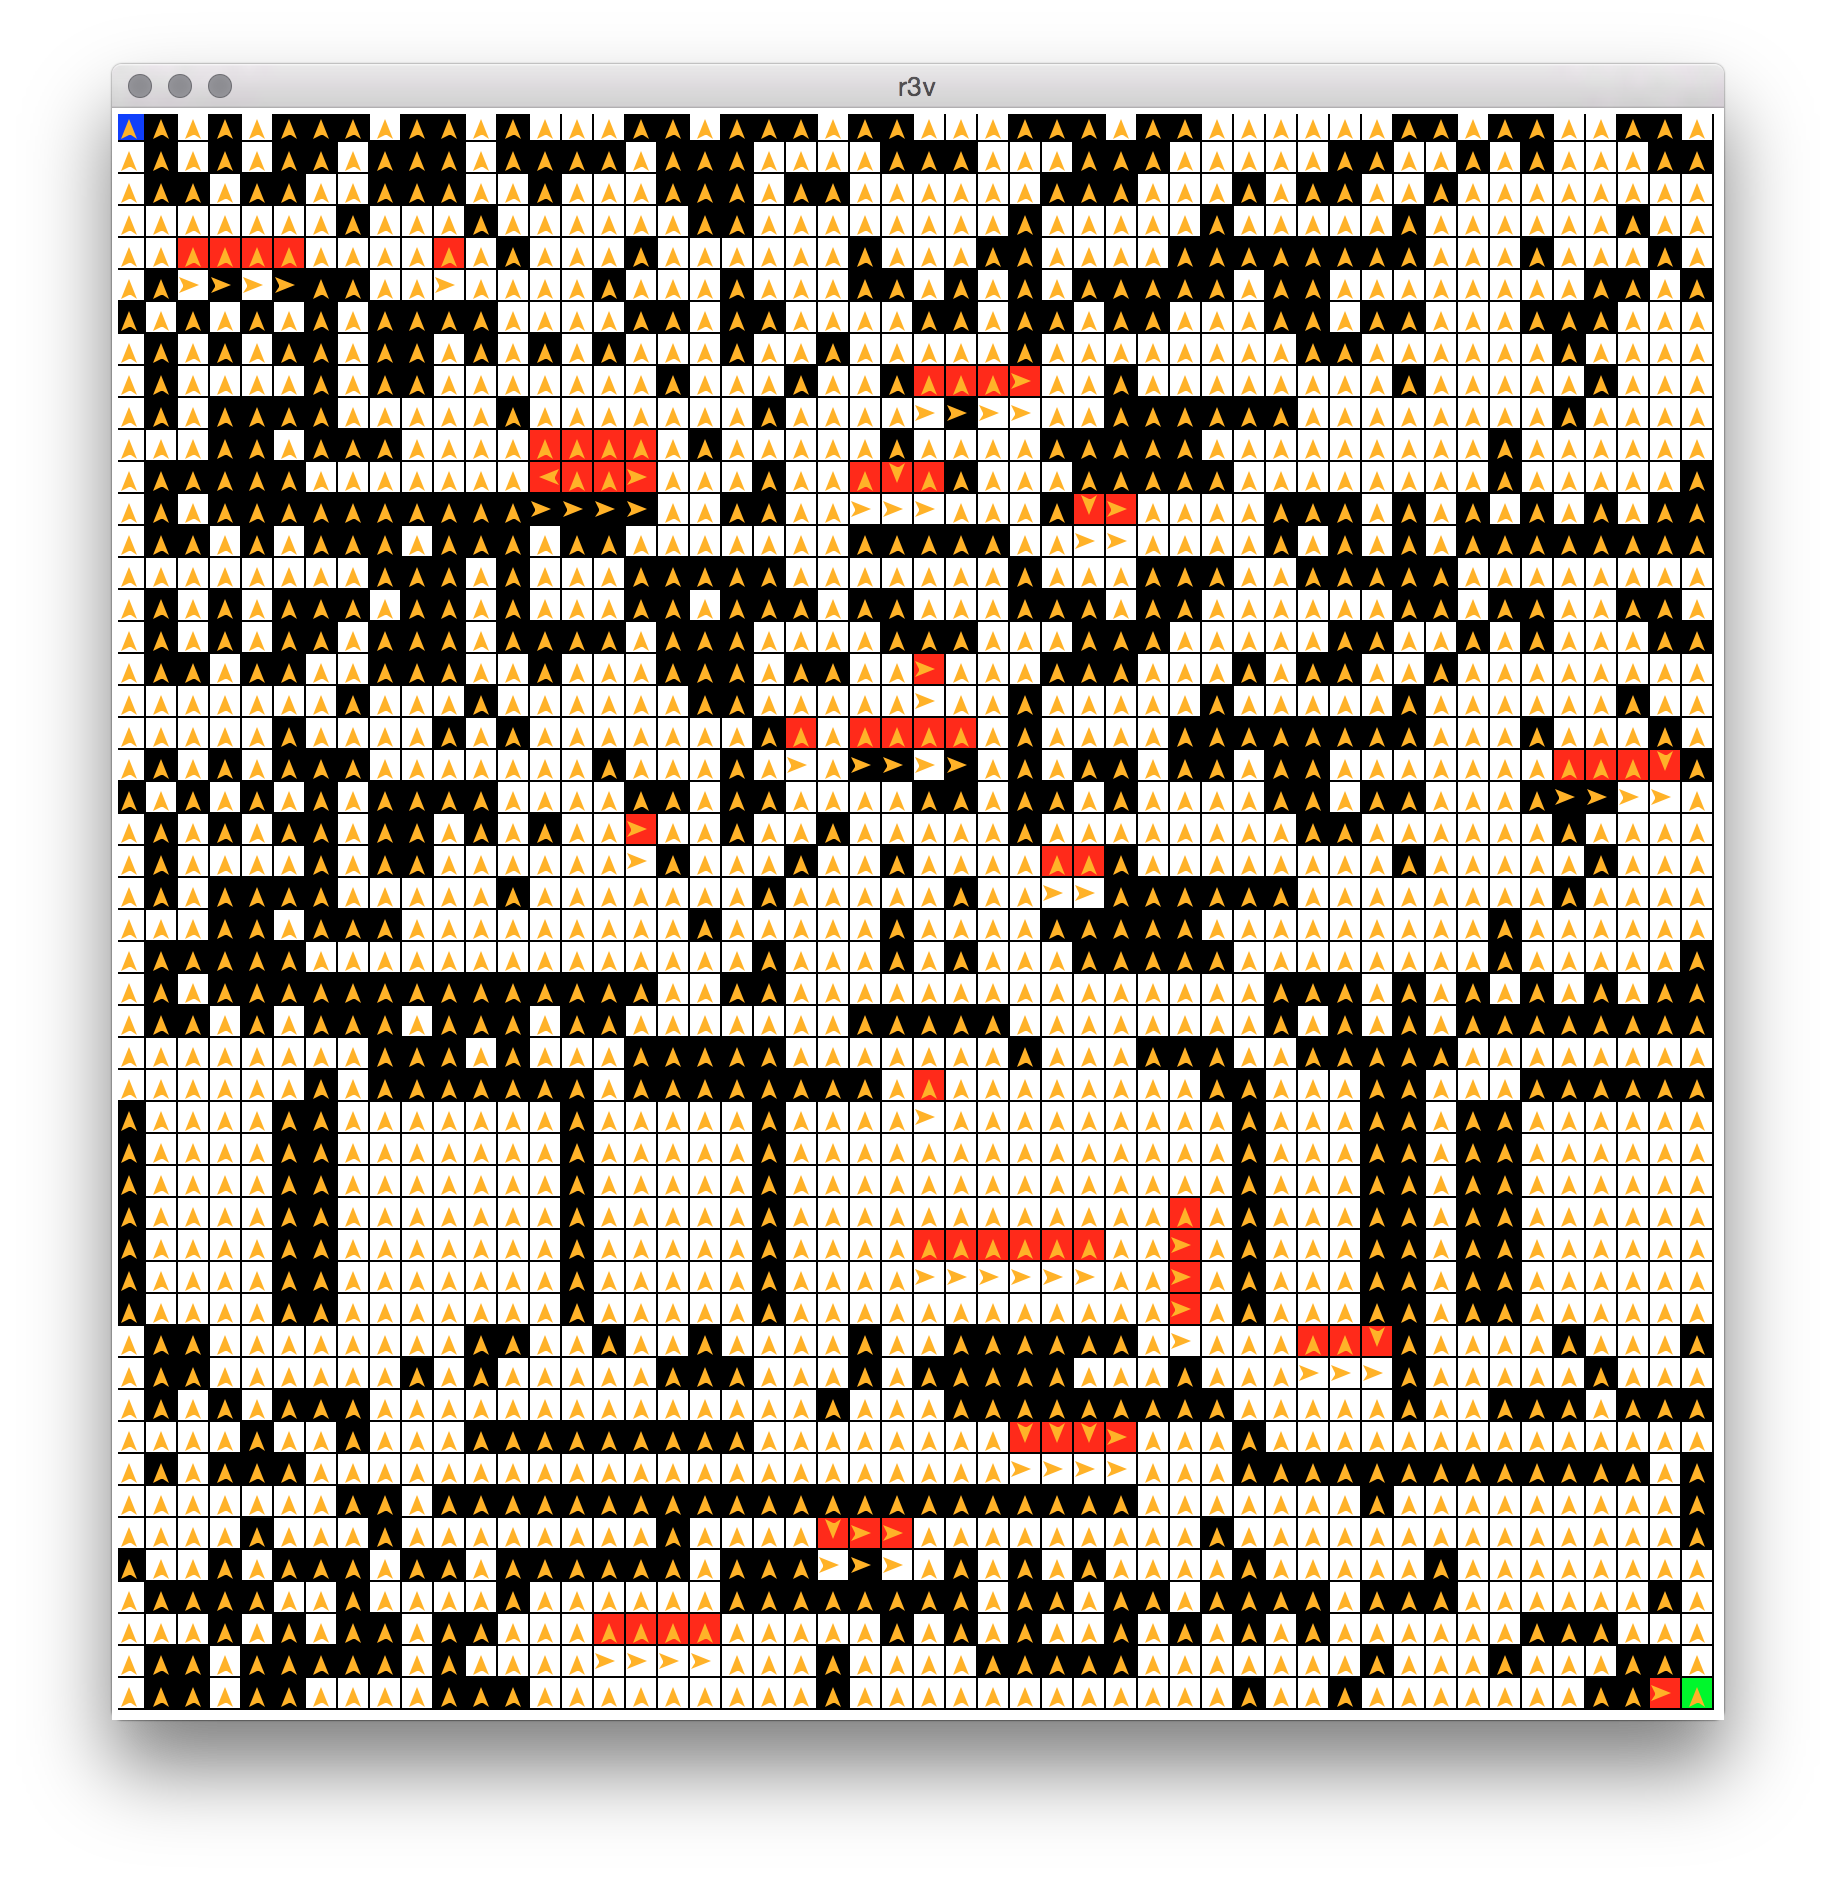
\includegraphics[width=\textwidth]{figures/50x50_v_r3.png}
                \caption{Reward schema 3\\
                Reward: $\infty$  \\
                Time:  0.03668\\
                Iterations: 3}
                \label{fig:v6}
        \end{subfigure}
        \caption{Policies Learned by Value Iteration}\label{fig:animals}
\end{figure}

Value iteration seemed to be able to get the correct optimal policy very quickly and in relatively few iterations. The times listed in \textit{Figure \ref{fig:v6}} do not include the time to build $T(s, a, s')$ or $R(s, a)$. The time need to construct this model was much greater than the time needed to find the optimal policy.

\subsubsection{Policy Iteration}
\begin{figure}[H]
        \centering
        \begin{subfigure}[b]{0.3\textwidth}
                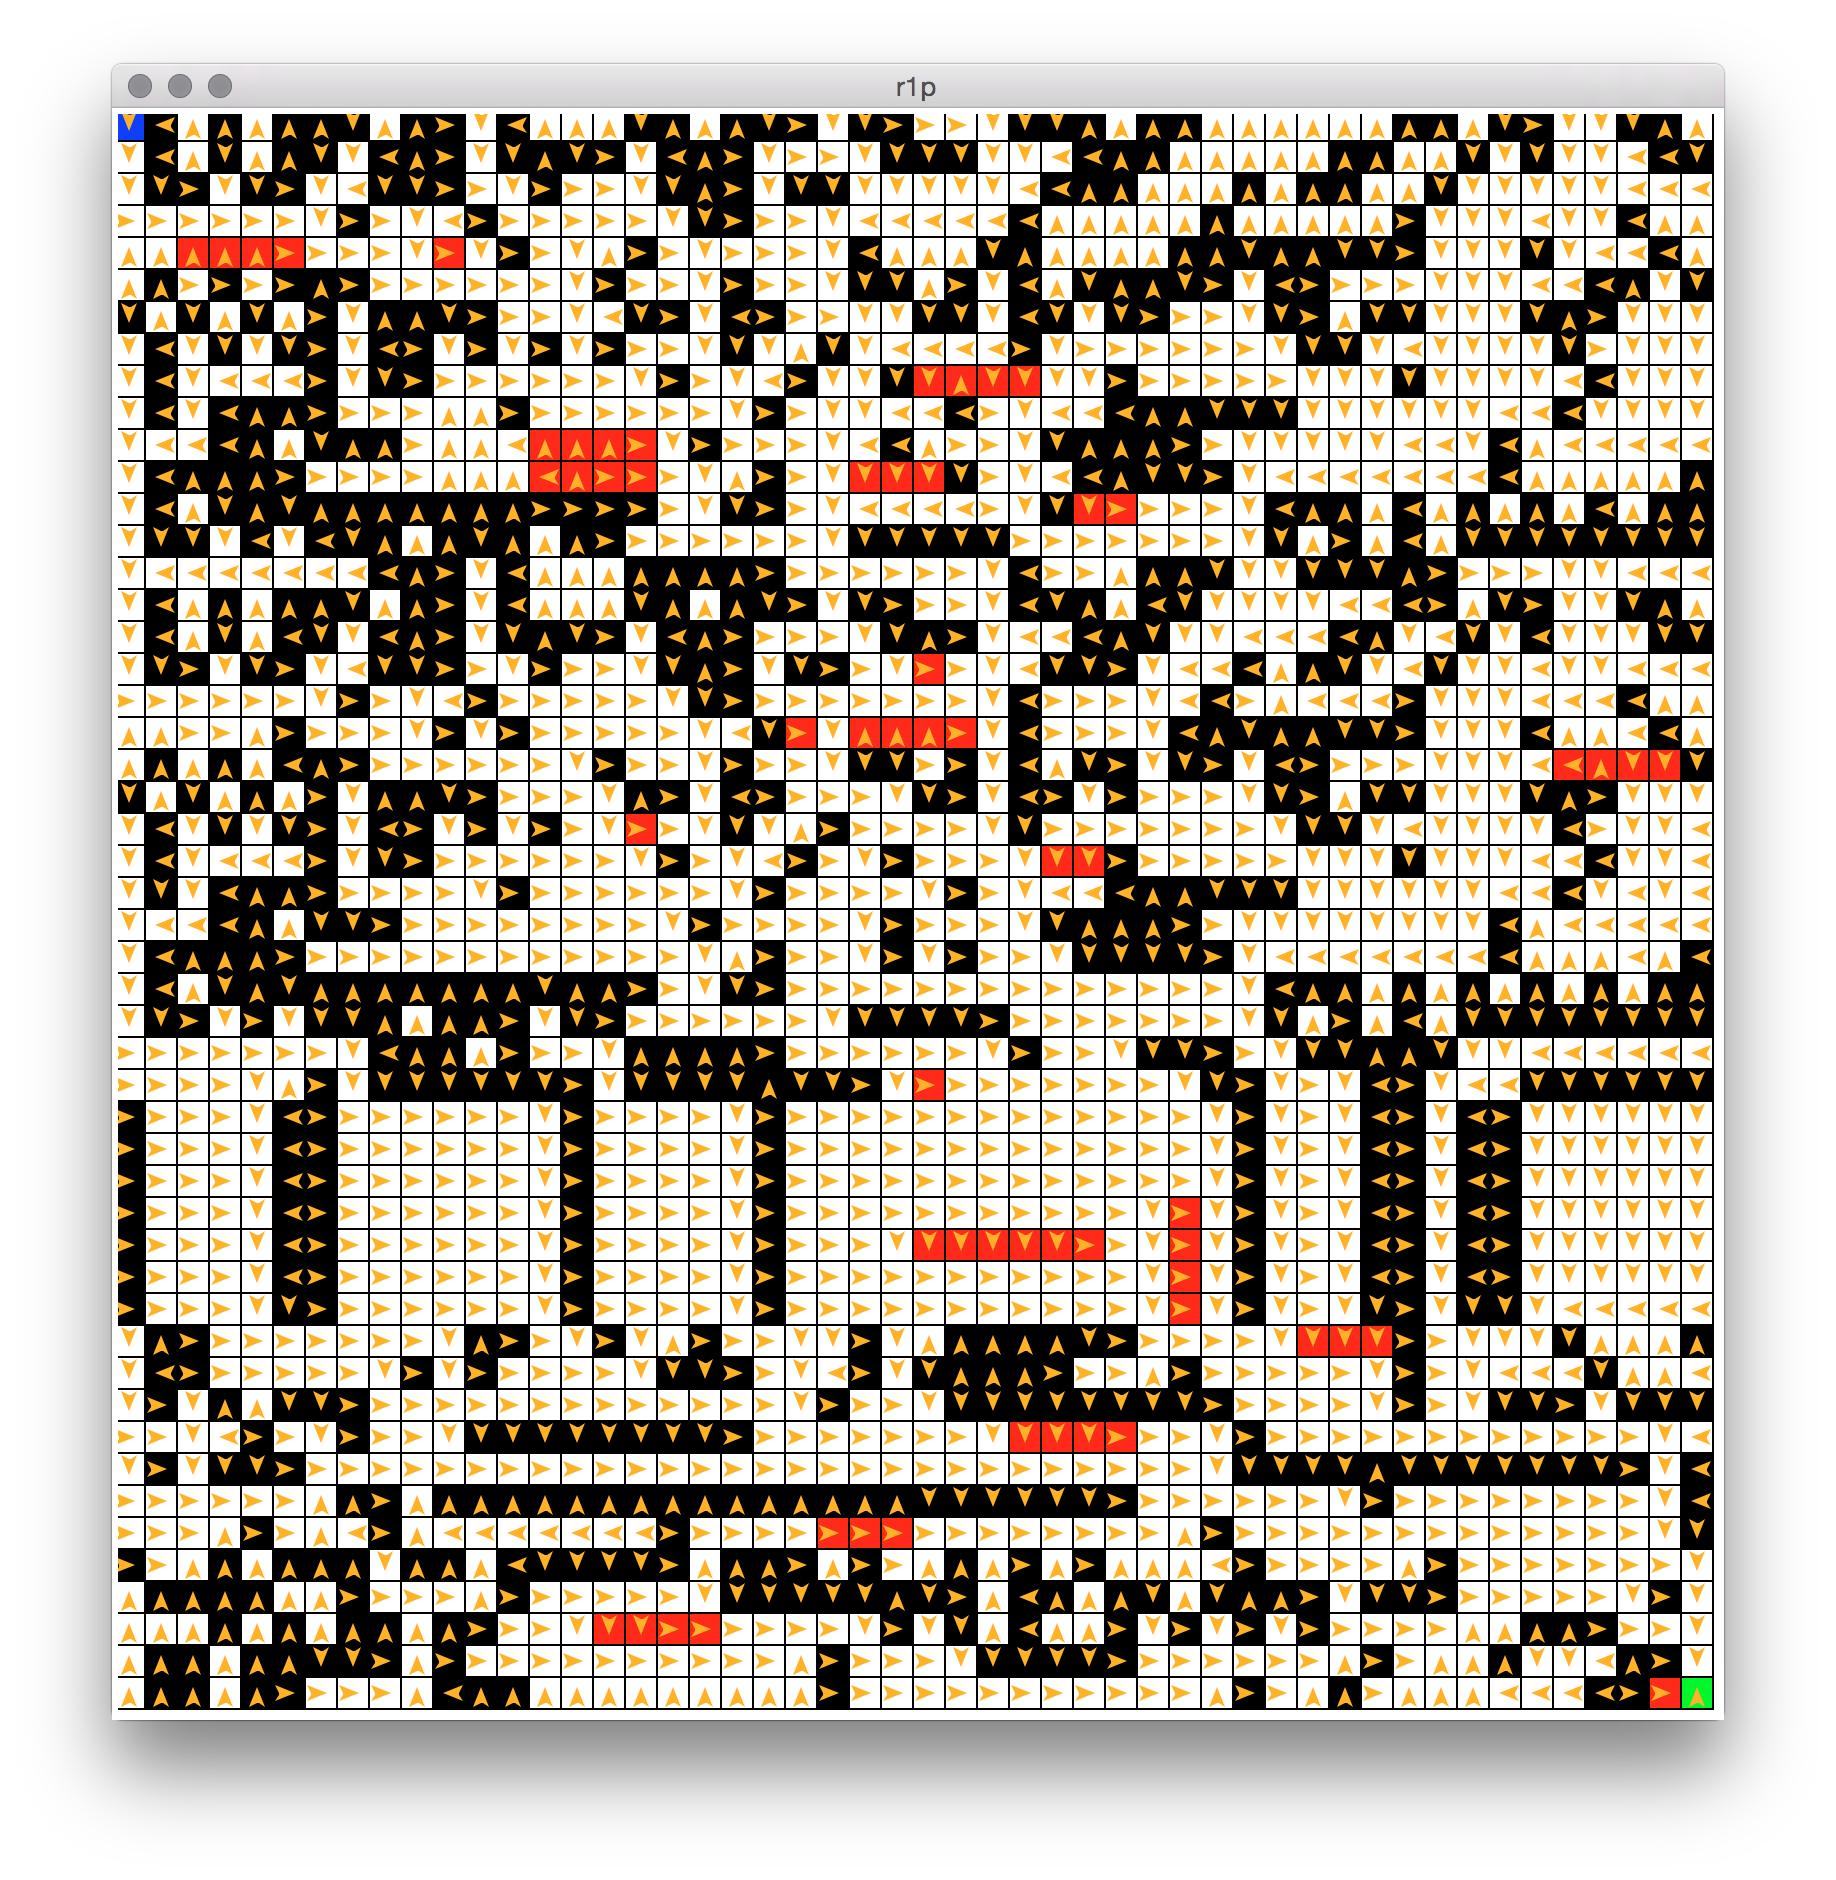
\includegraphics[width=\textwidth]{figures/50x50_p_r1.png}
                \caption{Reward schema 1\\
                Reward:  995.15 \\
                Time:  850.5694\\
                Iterations: 1000 (max)}
                \label{fig:gull}
        \end{subfigure}%
        ~ %add desired spacing between images, e. g. ~, \quad, \qquad, \hfill etc.
          %(or a blank line to force the subfigure onto a new line)
        \begin{subfigure}[b]{0.3\textwidth}
                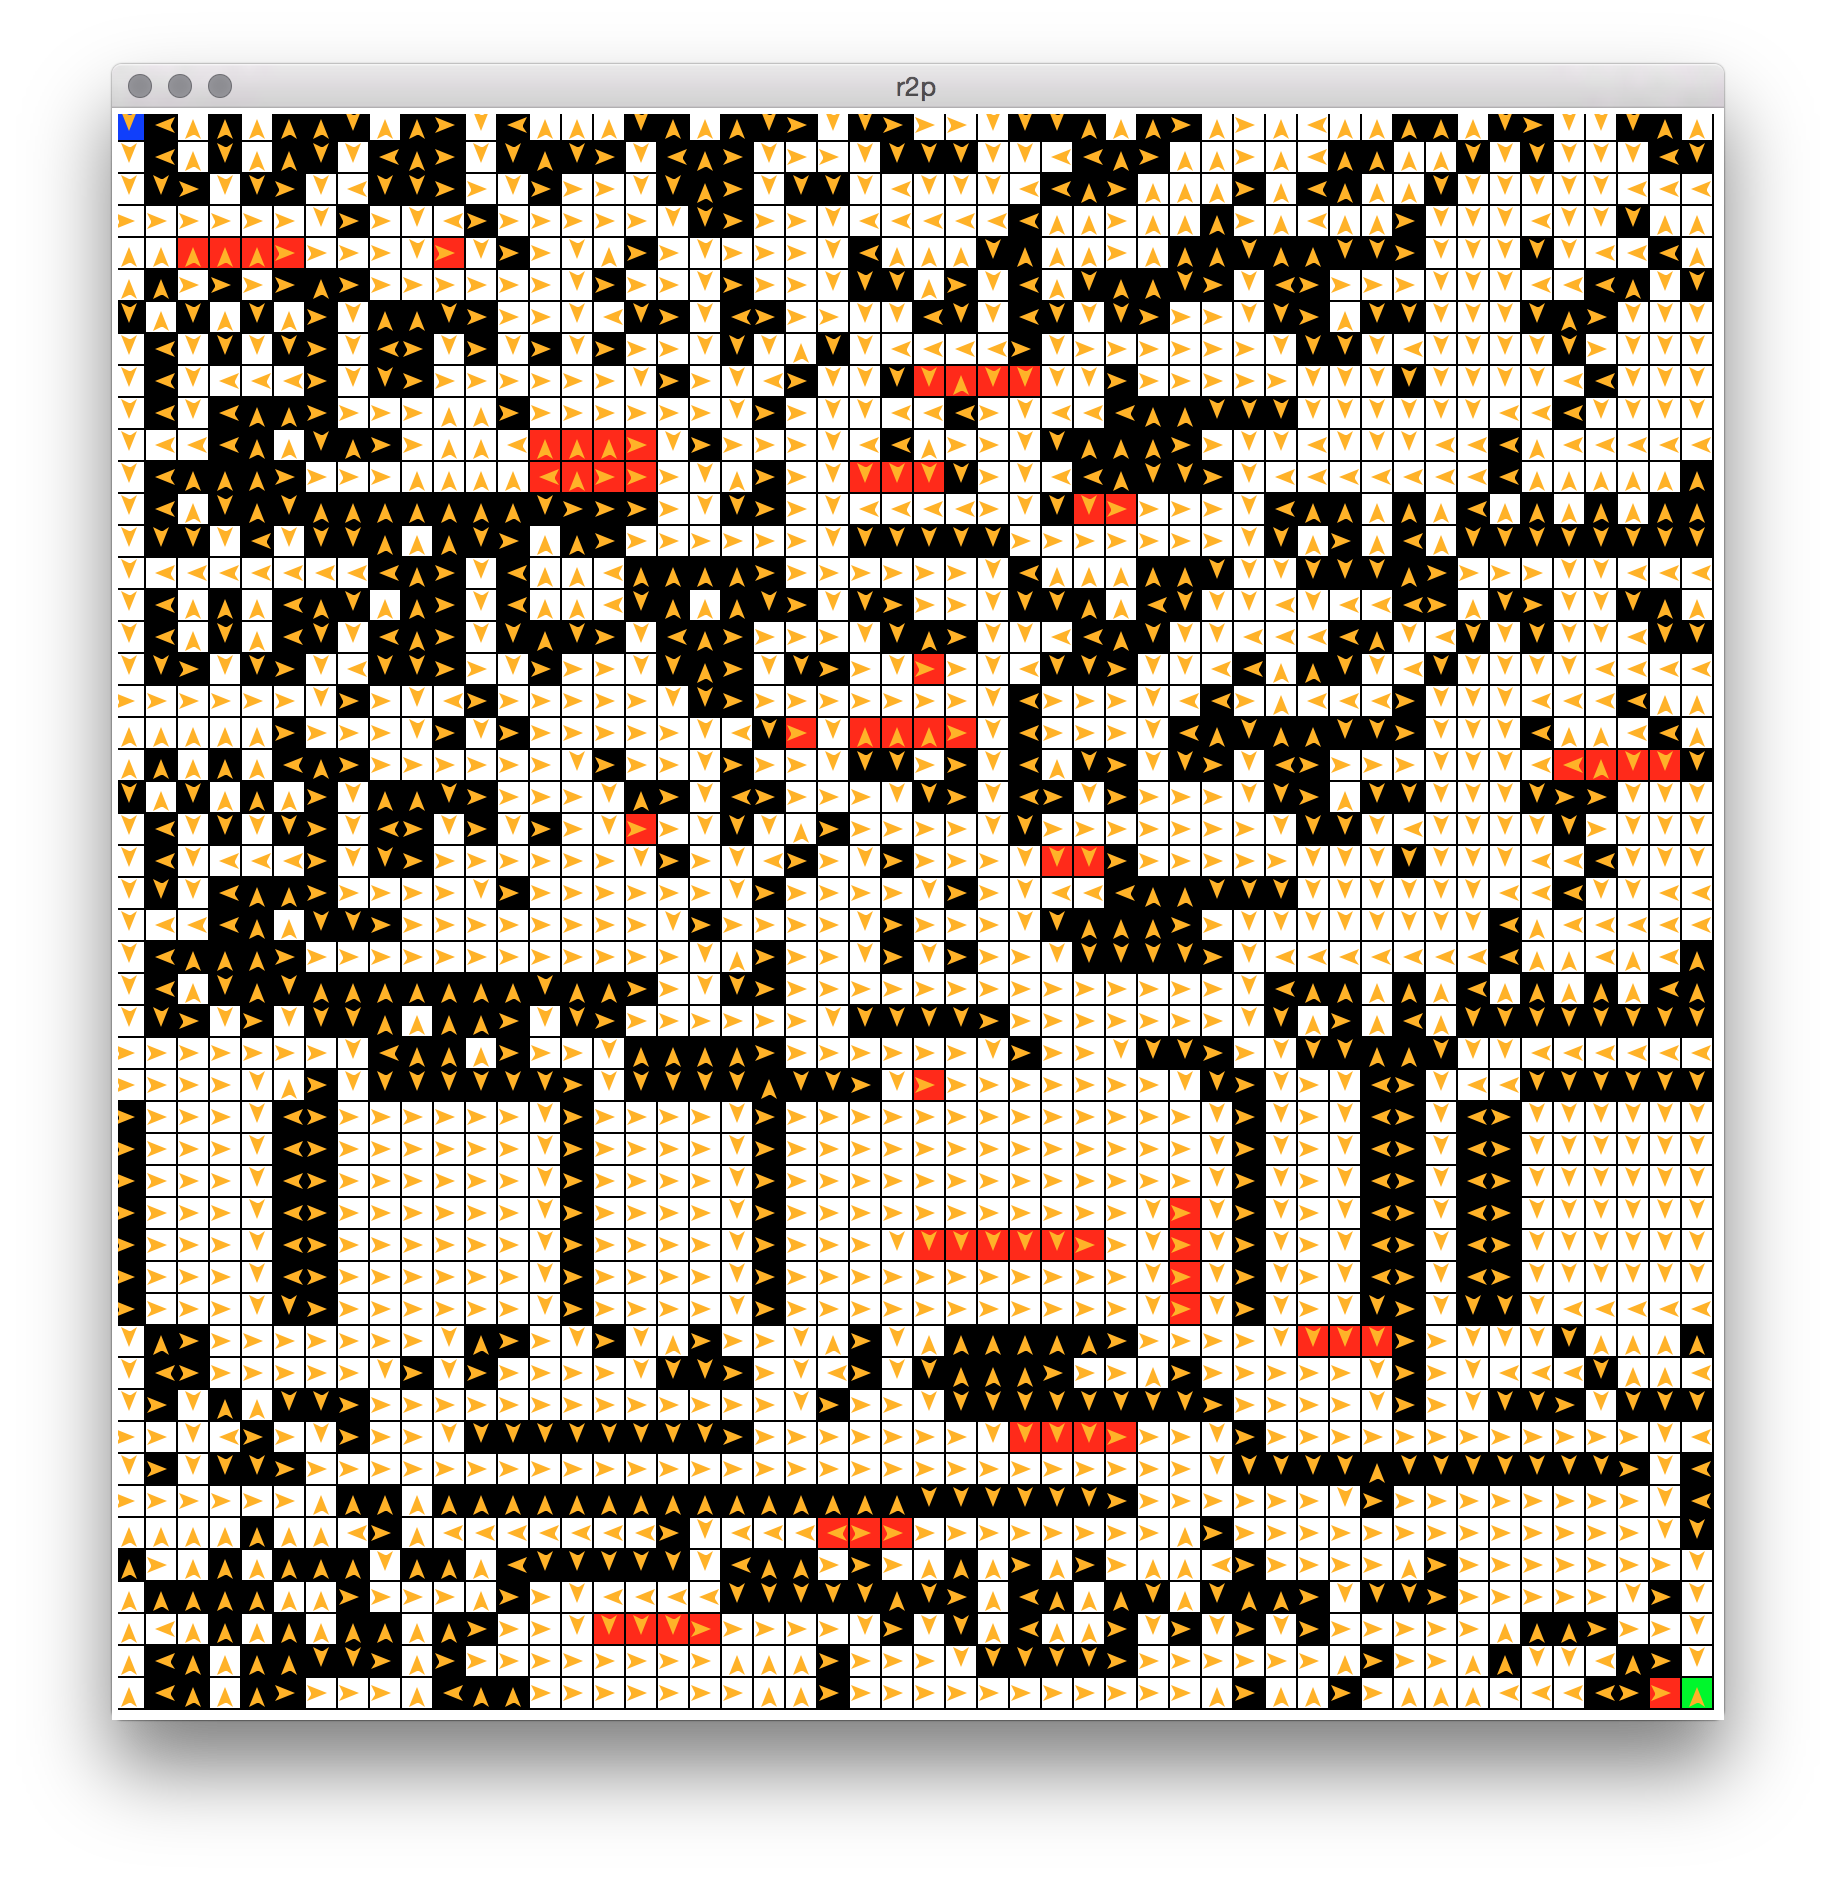
\includegraphics[width=\textwidth]{figures/50x50_p_r2.png}
                \caption{Reward schema 2\\
                Reward: 515 \\
                Time:  880.0052\\
                Iterations: 1000 (max) }
                \label{fig:tiger}
        \end{subfigure}
        ~ %add desired spacing between images, e. g. ~, \quad, \qquad, \hfill etc.
          %(or a blank line to force the subfigure onto a new line)
        \begin{subfigure}[b]{0.3\textwidth}
                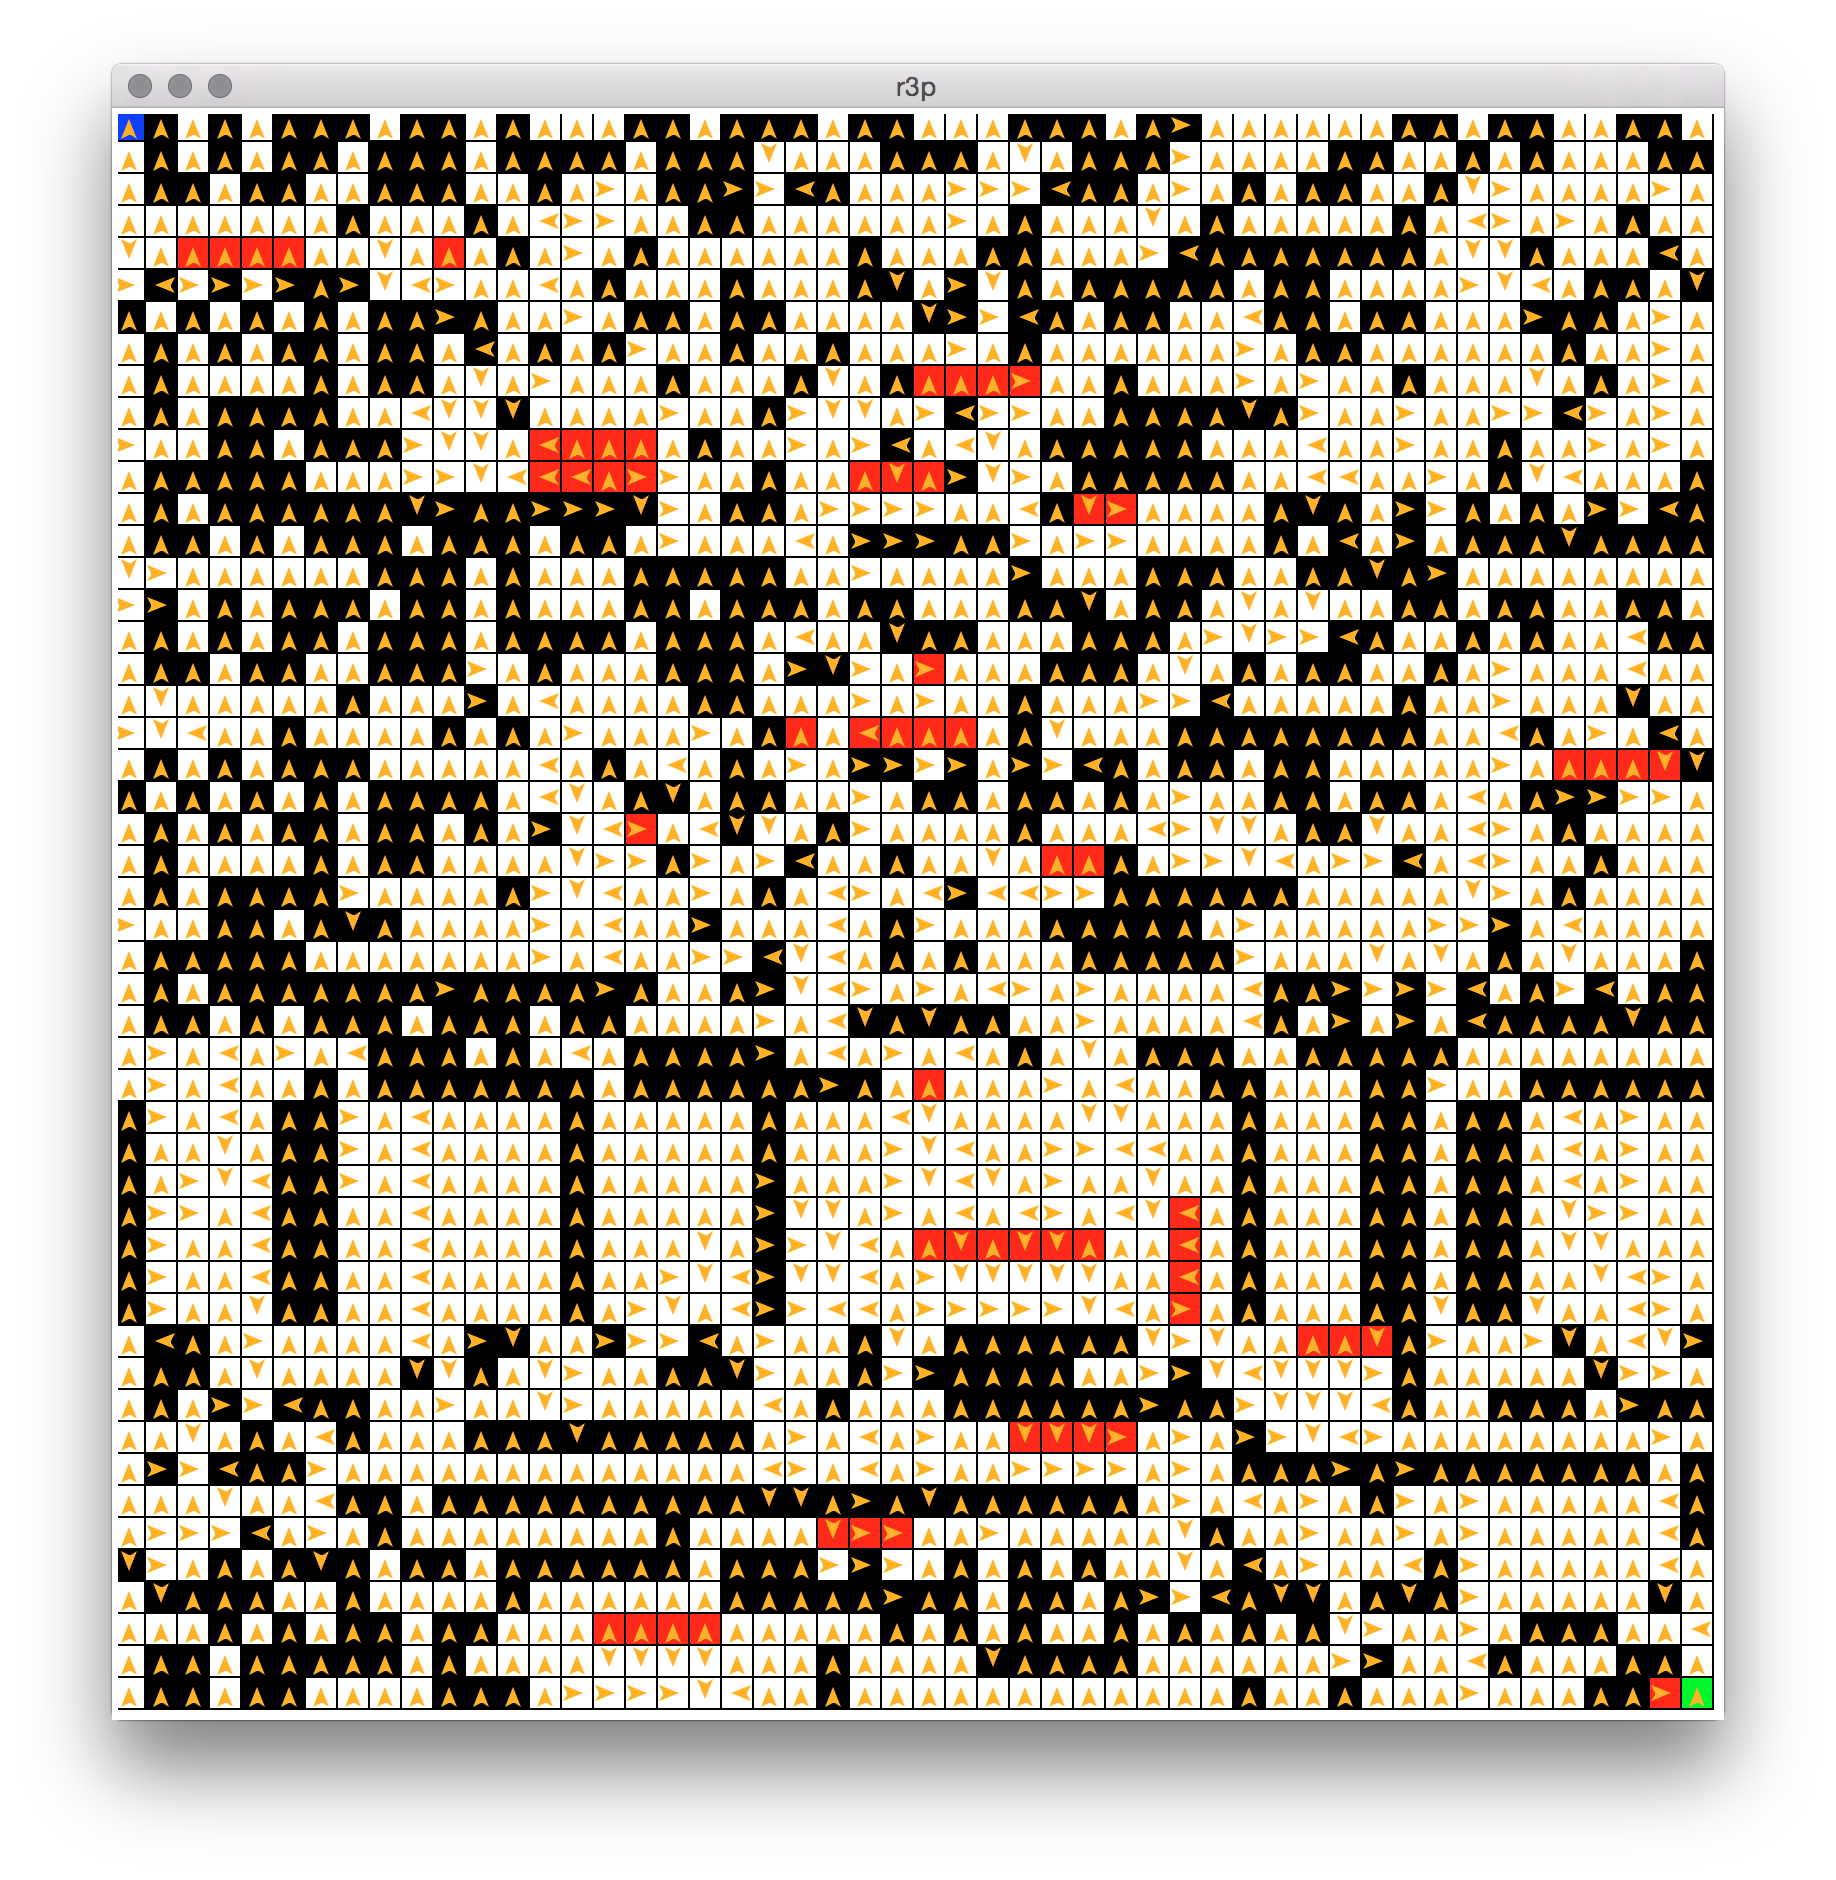
\includegraphics[width=\textwidth]{figures/50x50_p_r3.png}
                \caption{Reward schema 3\\
                Reward: $\infty$ \\
                Time: 846.6438\\
                Iterations: 1000 (max)}
                \label{fig:mouse}
        \end{subfigure}
        \caption{Policies Learned by Policy Iteration}\label{fig:animals}
\end{figure}

Policy iteration was also able to find the correct optimal policy in all cases. However the results are much less impressive. Each run used the maximum number of iterations allowed to it. It's possible that the optimal policy was found much earlier than the one-thousandth iteration and policy iteration spent most of it's time trying to refine this.

\subsubsection{Q-Learning}
\begin{figure}[H]
        \centering
        \begin{subfigure}[b]{0.3\textwidth}
                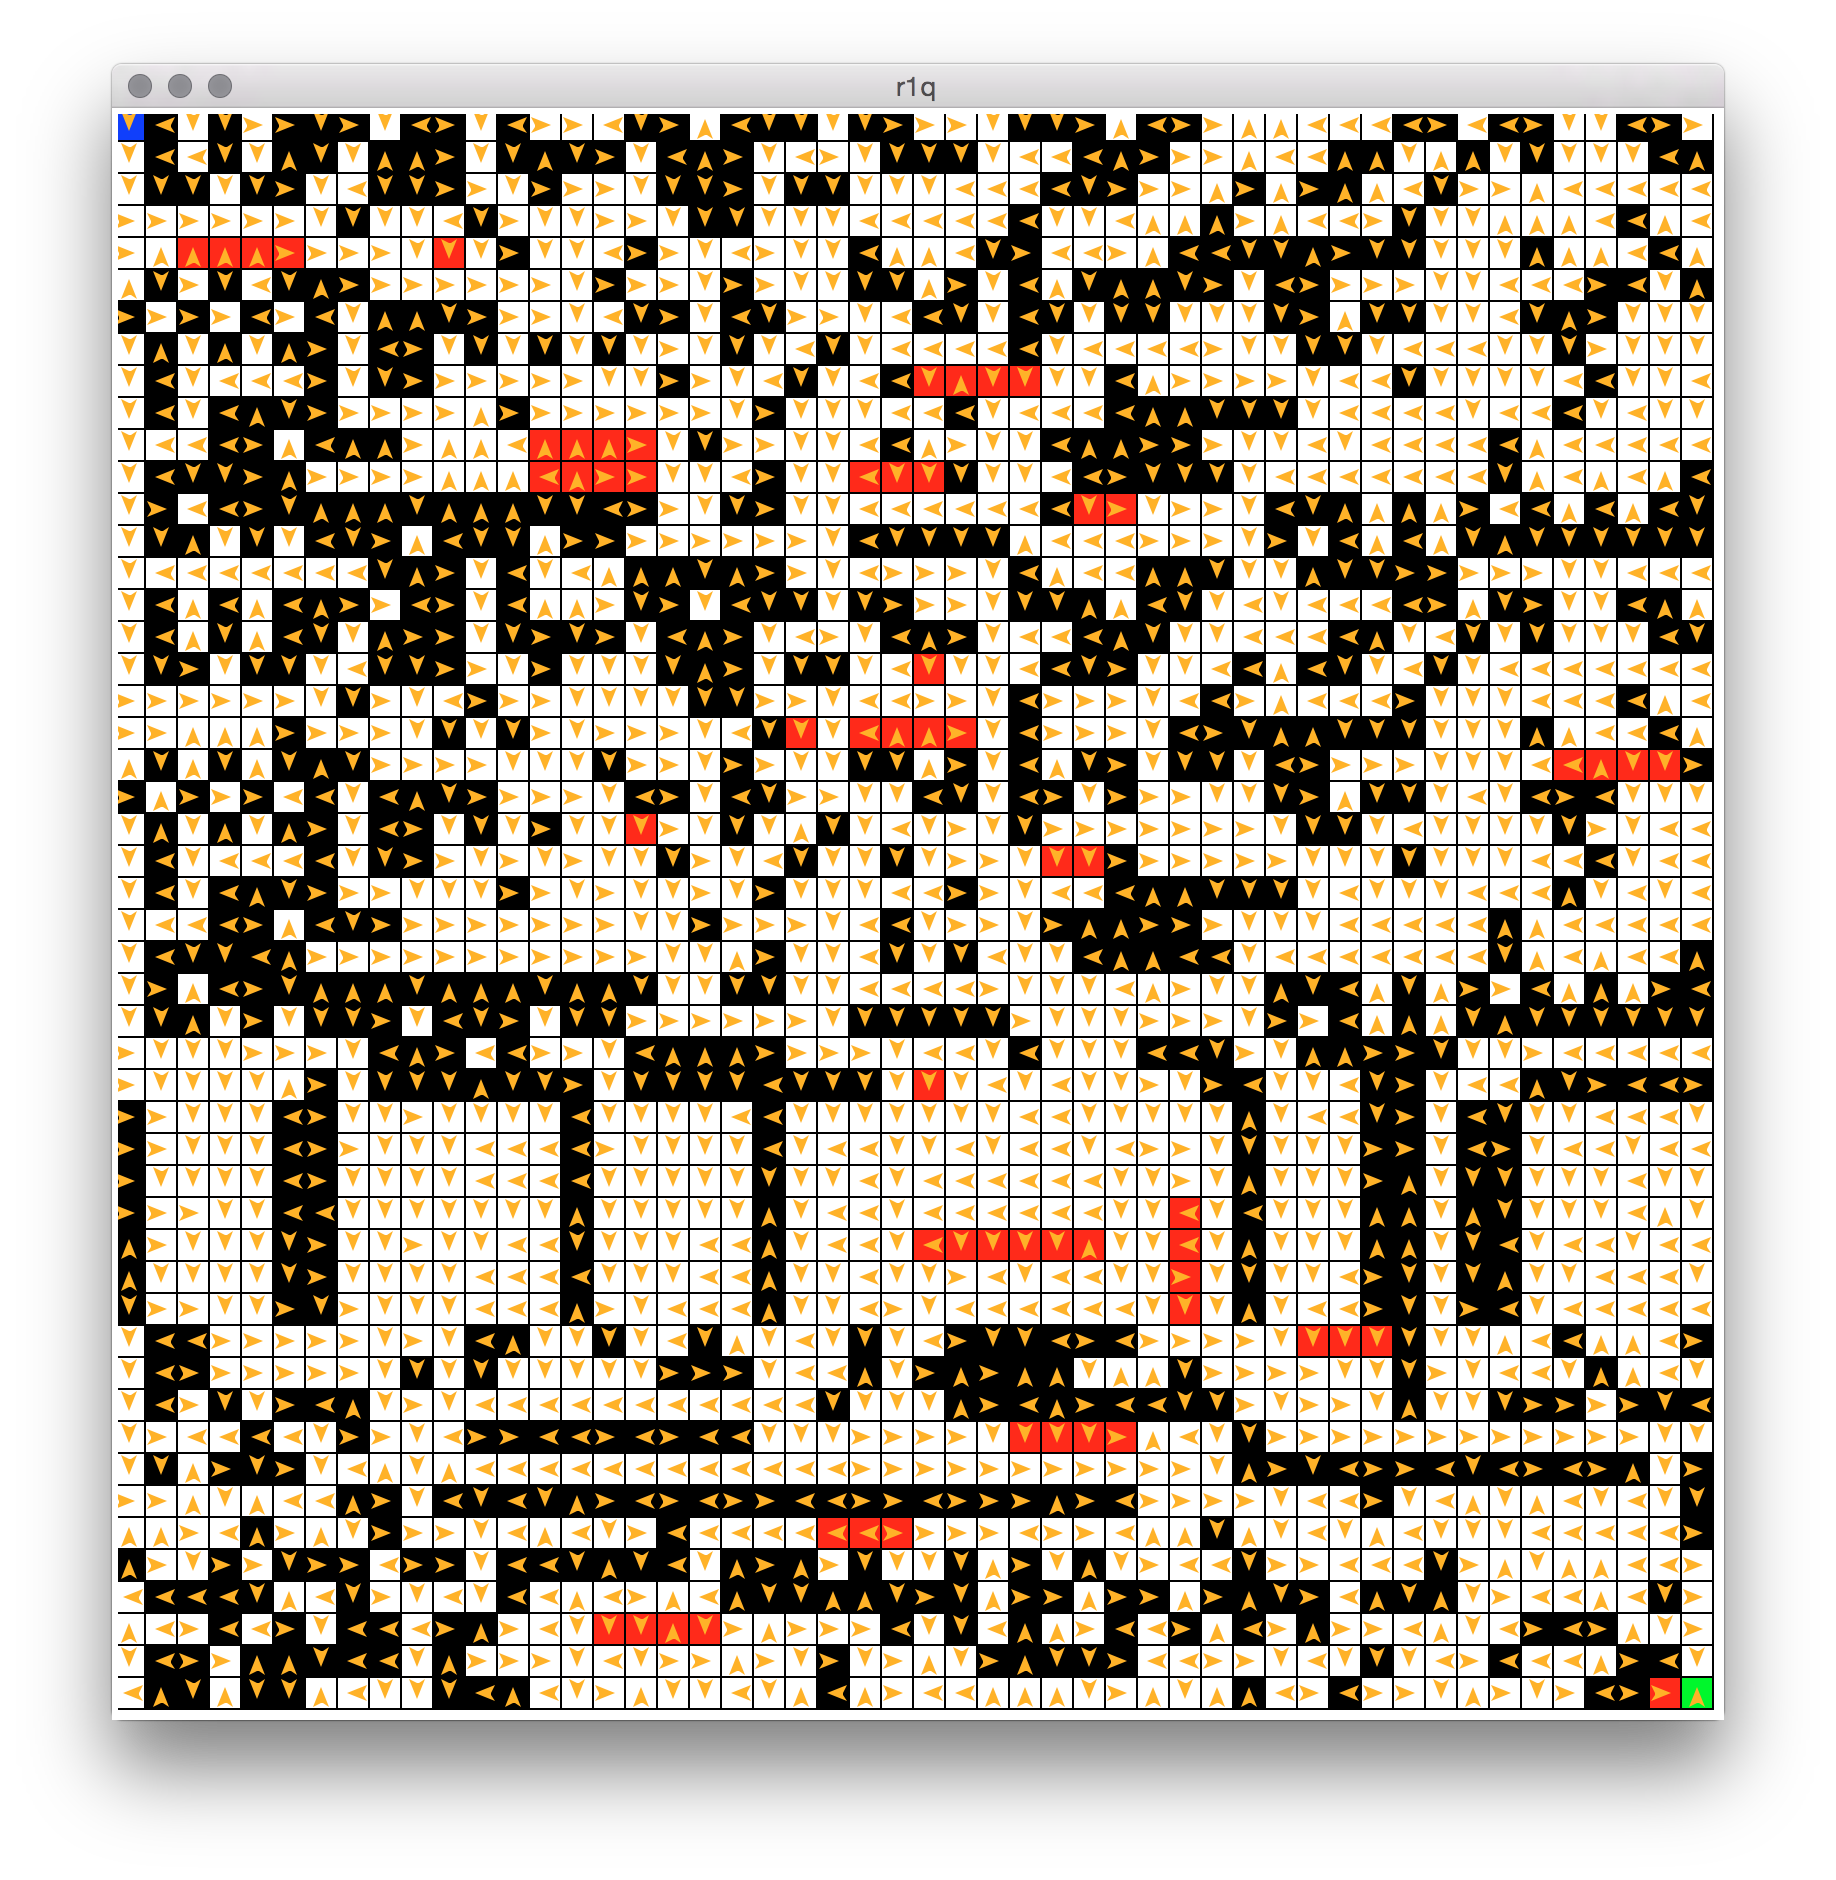
\includegraphics[width=\textwidth]{figures/50x50_q_r1.png}
                \caption{Reward schema 1\\ 
                Reward:  $\infty$ \\
                Time:  1443.6557 \\
                Iterations:  7493022 }
                \label{fig:qr1}
        \end{subfigure}%
        ~ %add desired spacing between images, e. g. ~, \quad, \qquad, \hfill etc.
          %(or a blank line to force the subfigure onto a new line)
        \begin{subfigure}[b]{0.3\textwidth}
                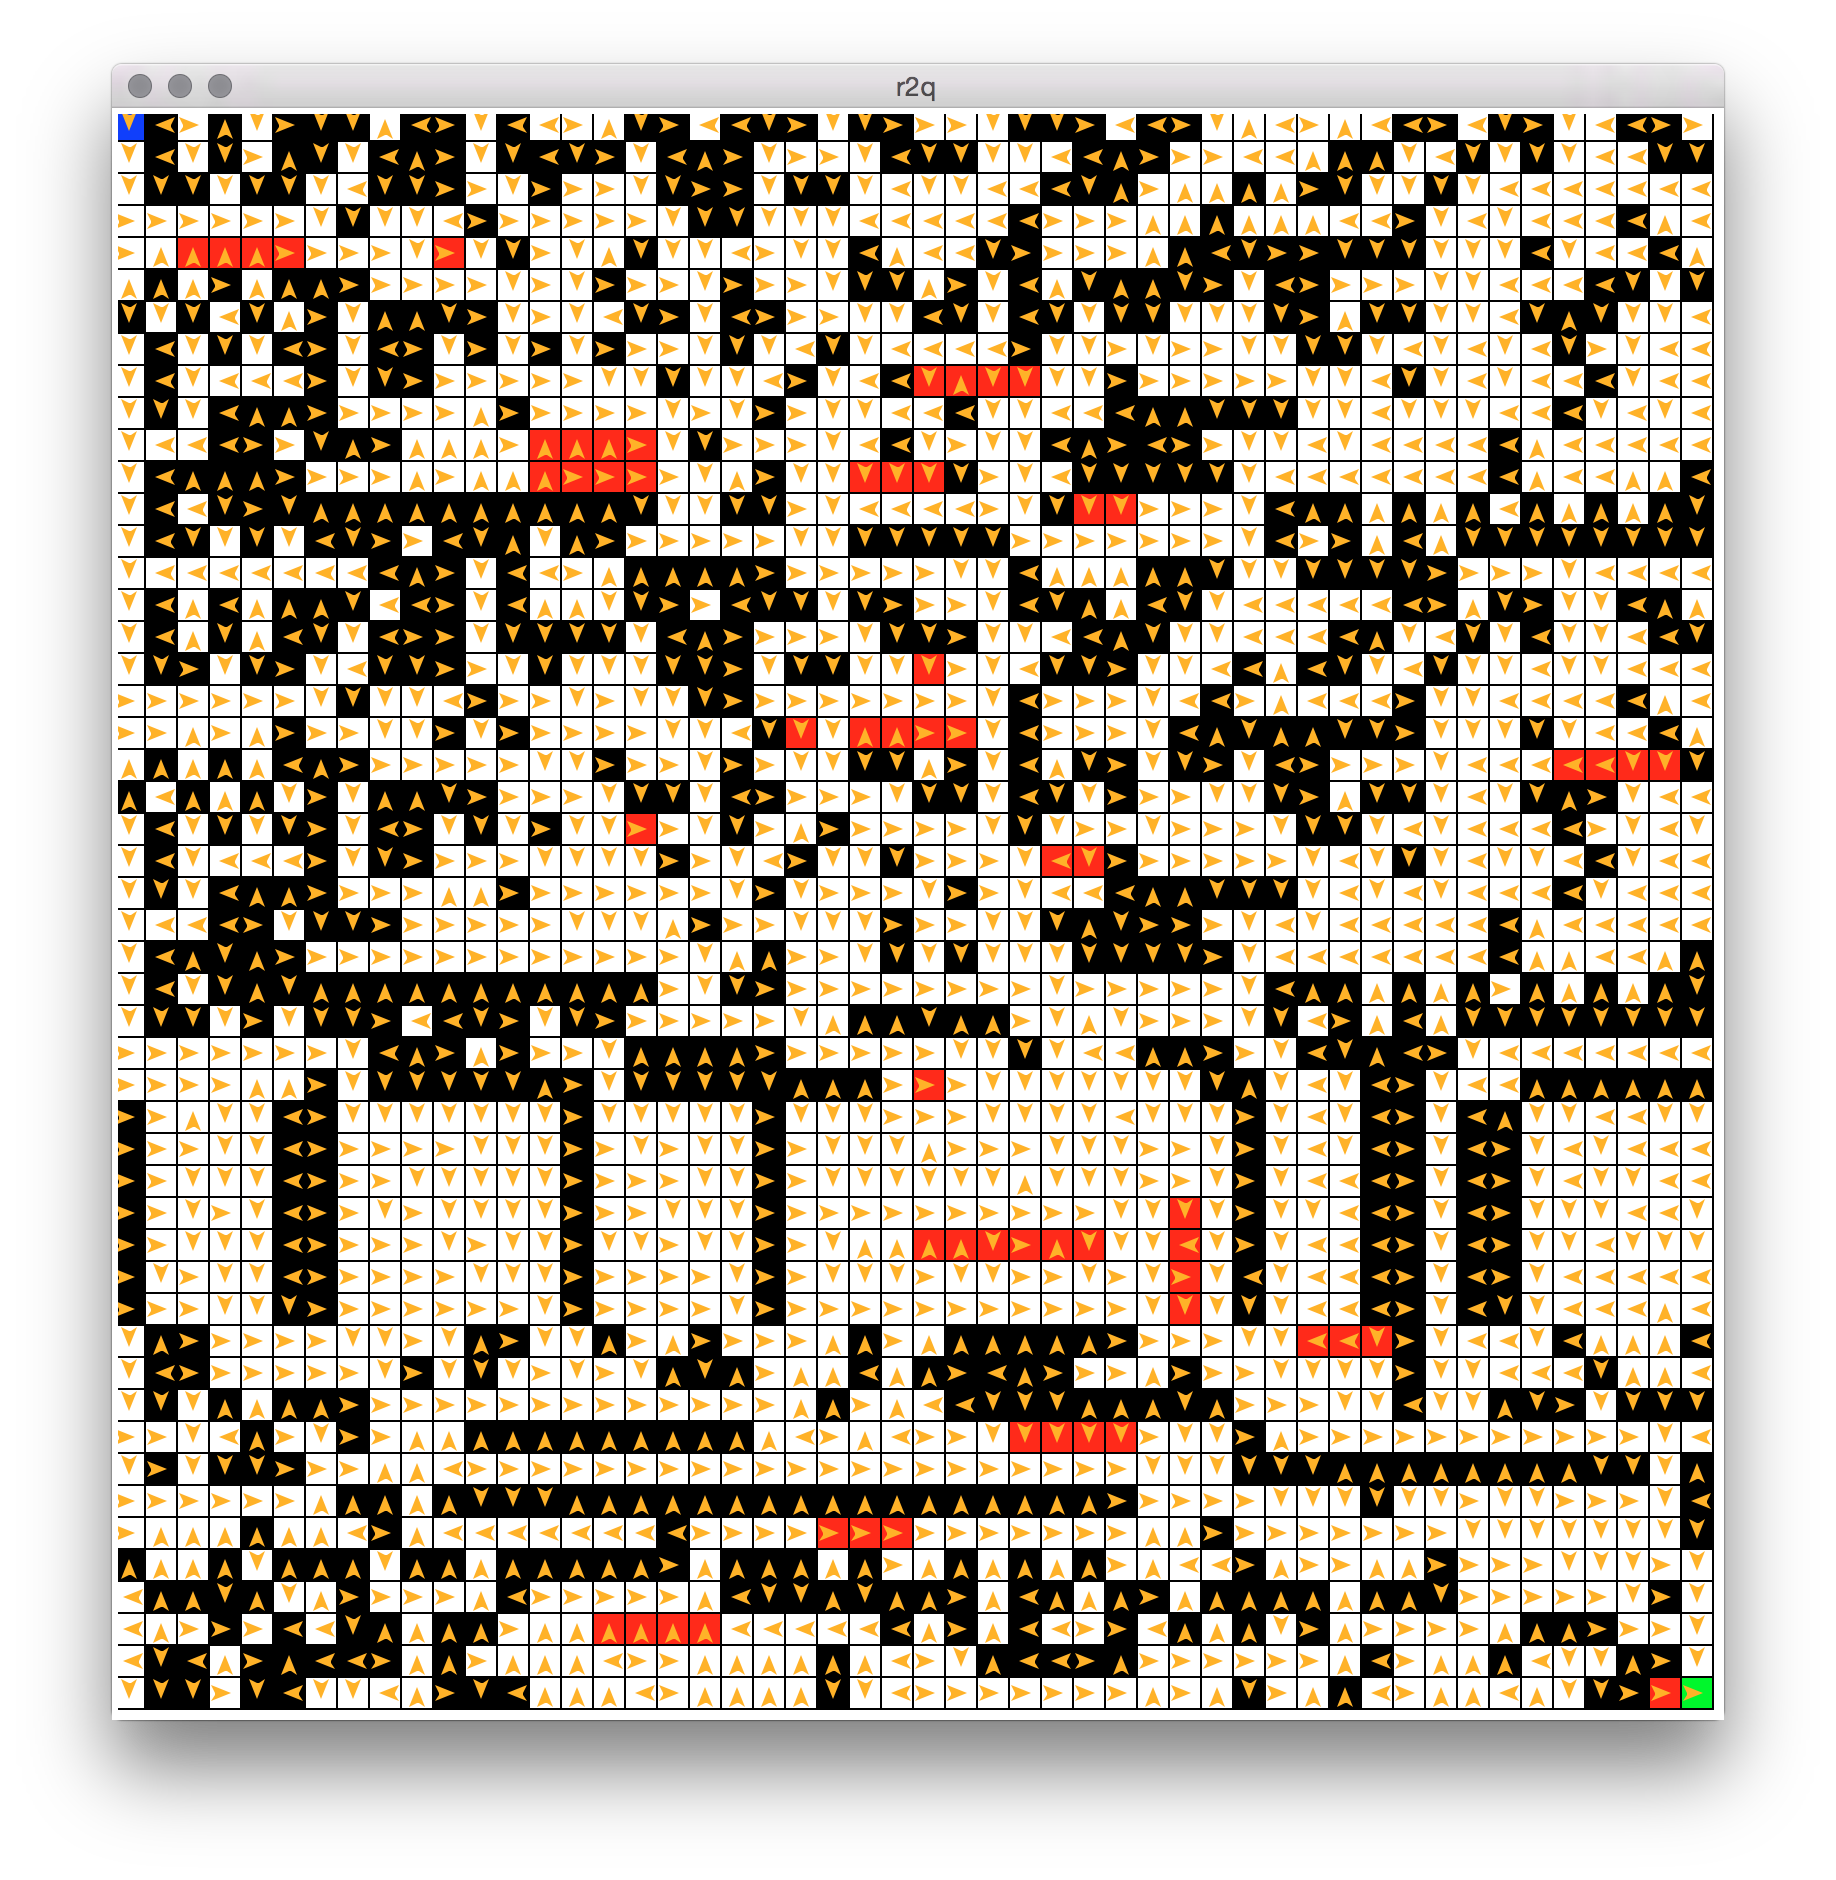
\includegraphics[width=\textwidth]{figures/50x50_q_r2.png}
                \caption{Reward schema 2\\
                Reward: 515\\
                Time:  2058.5023\\
                Iterations: 11688558 }
                \label{fig:qr2}
        \end{subfigure}
        ~ %add desired spacing between images, e. g. ~, \quad, \qquad, \hfill etc.
          %(or a blank line to force the subfigure onto a new line)
        \begin{subfigure}[b]{0.3\textwidth}
                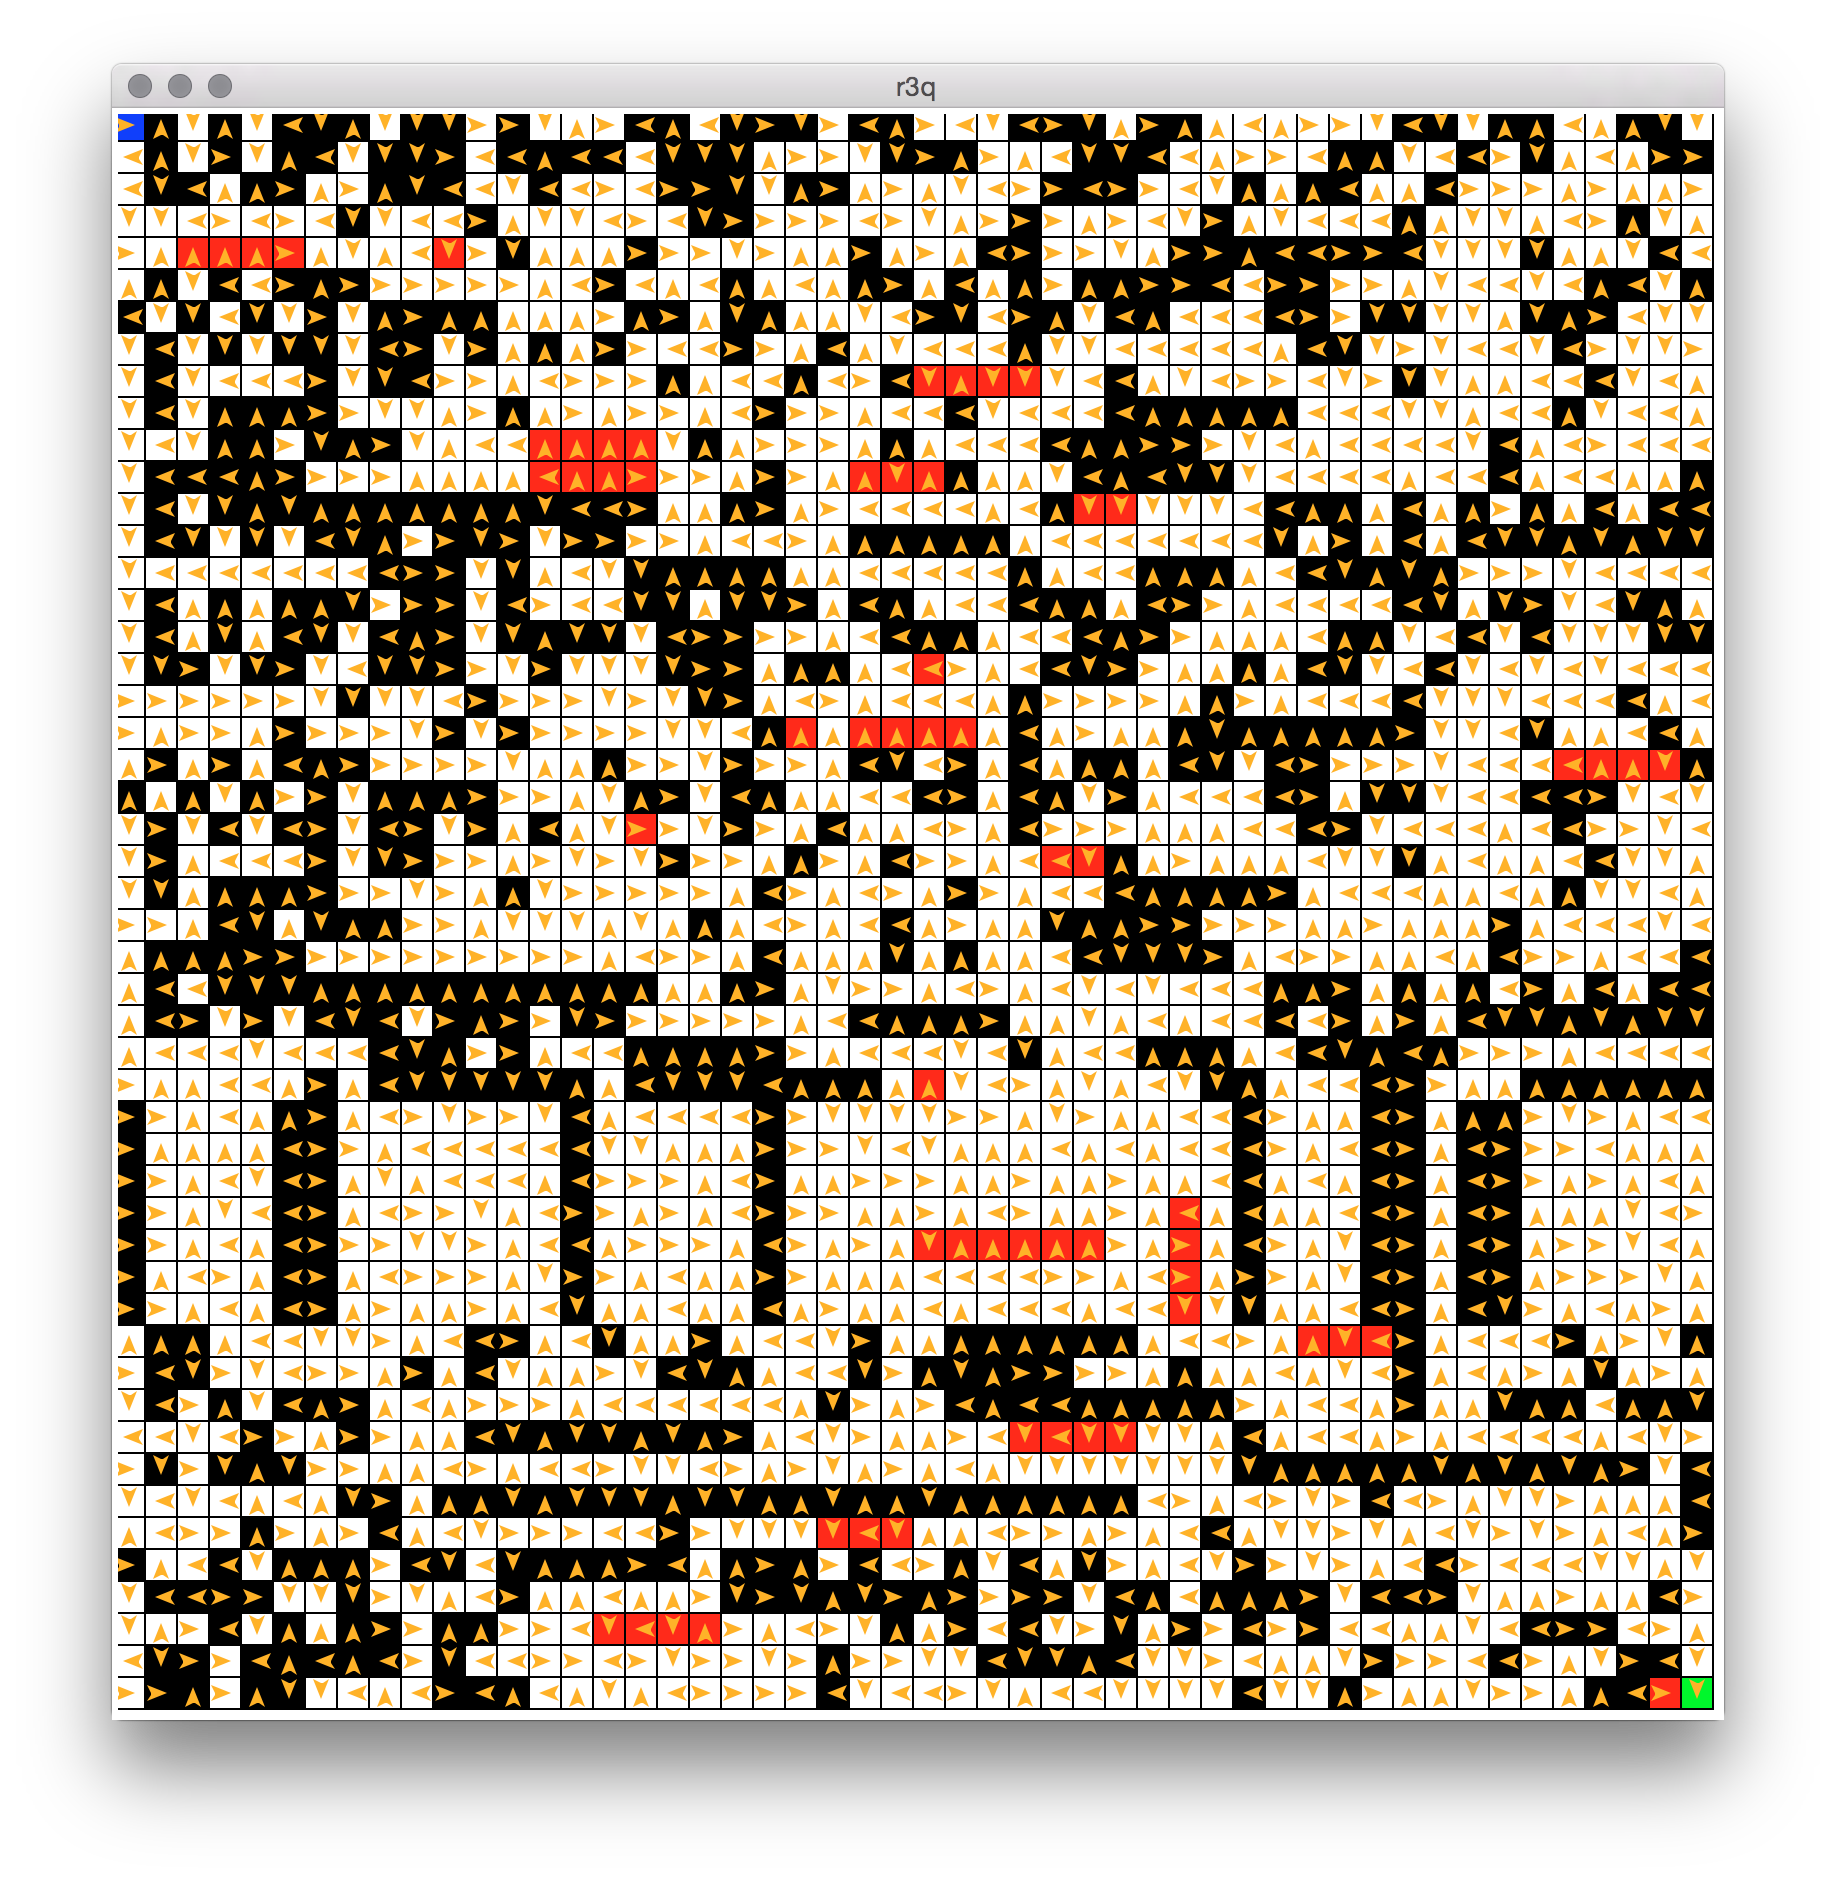
\includegraphics[width=\textwidth]{figures/50x50_q_r3.png}
                \caption{Reward schema 3 \\
                Reward: $\infty$\\
                Time: 1745.3181 \\
                Iterations: 9459882 }
                \label{fig:mouse}
        \end{subfigure}
        \caption{Policies Learned by Q-Learning}\label{fig:animals}
\end{figure}

In \textit{Figure \ref{fig:qr1}}, Q-learning was unable to find the optimal policy. This seems to be the effect of size of the step penalty. \textit{Figure \ref{fig:qr2}} had a larger step penalty that was able to encourage the agent to quickly find a path to the goal and hence achieve the correct result.

In all cases Q-learning took much longer than the methods in which the model was already known. This makes intuitive sense, since when given a model the agent is able to directly look up the consequences of future actions. 

\section{Conclusion}

For model-based methods value iteration was able to outperform policy iteration in terms of speed. This is most probably due to the computational intensity of each of policy iteration's iterations where it needed to solve a system of linear equations in order to update the policy. In straightforward cases, however, policy iteration was able to converge in many fewer iterations than value iteration. In non-straightforward cases (such as those where the terminal state gives no positive reward), it seemed that value iteration was able to more quickly find the optimal policy.

Q-learning, in all cases, took longer than either of the model-based methods. This makes intuitive sense, since the model based methods were able to easily look ahead to discover future reward sequences whereas Q-learning had to rely on exploration. However, Q-learning is still probably a more commonly useful approach. Knowing the model and reward function may be unlikely in real world scenarios, and when they are known it is often improbable to store them in memory. The 50x50 gridworld was the "large" problem presented in this paper, however it  only contained 2500 states. With 2500 states the size of the transition probability matrix was $4\times2500\times2500 = 25,000,000 $ elements. 

\begin{center}
\noindent\rule{8cm}{0.4pt}
\end{center}

[1] Kaelbling, Leslie Pack \& Littman, Michael L \& Moore, Andrew W (1996). Reinforcement Learning: A Survey. Journal of Artificial Intelligence Research 4. 237-285

[2] Watkins, C.J.C.H (1989). Learning from Delayed Rewards. Ph.D. thesis, Cambridge University

\end{document}